% !Mode:: "TeX:UTF-8"
\chapter{基于\texorpdfstring{\(^{18}\)}{18}F-FDG PET/CT三维影像的下肢骨折相关感染检测与诊断框架}

上一章介绍了应用于骨三相中进行骨科相关感染诊断的人工智能方法,本章将根据PET/CT影像中骨科相关感染的诊断流程,研究患者下肢的骨折相关感染(Fraction-Related Infection)的检测与诊断,并提出了全自动两阶段的下肢骨折相关感染检测与诊断框架。第一阶段通过双分支三维定位网络检测病灶区域,第二阶段通过卷积神经网络进一步地进行病灶分类,预测是否存在感染。检测部分通过PET主分支和CT辅分支的网络结构设计有效地提取两种不同模态的特征并进行逐阶段地充分融合生理代谢信息和解剖组织信息。诊断分类部分对检测的病灶进行最大强度投影转换为二维影像,在降低数据和模型规模的同时保留有效特征,通过分类器计算得到预测结果。该方法可以较为准确地检测出病灶并拥有较高的诊断分类准确率。

\section{问题分析}


在应对PET/CT三维影像中下肢骨折相关感染的诊断任务时,需综合考虑医生对于骨折相关感染的诊断流程、PET/CT影像的特性,以及人工智能在该诊断任务中的应用可能面临的挑战,可以概括如下:

(1)\textbf{缺乏关于下肢骨折相关感染的公开数据集}。目前网络上暂无公开的关于骨折相关感染的数据集。由此,本文作者与上海市第六人民医院核医学科医生合作收集了来源于真实患者下肢的PET/CT影像,并构建了与真实分布一致的下肢骨折相关感染的PET/CT影像多模态数据集。然而,数据集整体规模相对较小,而且在类别上分布不平衡。\textbf{这种数据集的特性对于模型的训练提出了额外的挑战}。

(2)\textbf{CT中骨折相关感染病灶的形状与分布区域多样}。在骨折相关感染的临床诊断流程中,首要任务是明确病变的具体位置。尽管骨折相关感染的病灶位置与骨骼强度相关,但由于人体骨骼广泛分布于全身,与一些组织和器官相比,并不像它们存在于一个相对固定的位置或者范围内。其次,病变的程度也有所差异,可能会涉及骨骼的不同部位以及软组织的破裂和损伤,也可能因个体差异而不同,导致病灶形状多变。因此,\textbf{对于骨折相关感染的病灶位置,是否能够准确地检测出至关重要}。

(3)\textbf{PET中高摄取区域呈现的形式和程度各不相同}。从核医学影像的角度分析,PET影像可以通过人体的组织细胞对于示踪剂氟代脱氧葡萄糖的摄取程度来展示人体的生理代谢信息。生理代谢强的区域一般都有着对于示踪剂的摄取程度高的特点,但呈现的形式与程度也各不相同。此外,人体中存在的自然高摄取区域(膀胱、肾脏等),以及炎症和愈合过程都会导致周围的软组织的摄取能力增加。骨折相关感染的病灶区域也因自身病变程度的不同而展示出各种不同的摄取形式和程度。因此,\textbf{如何避免其他高摄取区域造成的混淆是一个本章研究的主要问题}。

(4)\textbf{PET和CT影像之间不同的特征}。PET和CT是两种不同的医学影像模态,各自可以表现不同的内容信息。PET影像可以展现出人体的生理代谢信息,而CT影像可以展现出人体的解剖组织信息。同时,PET和CT均为三维影像。因此,\textbf{充分利用PET和CT影像的两种不同信息以及它们本身的三维性质同样是一个值得研究的问题}。

(5)\textbf{病灶检测中正负样本不平衡}。在本章的下肢骨折相关感染数据集中,一个病人一般仅有一个或二个病灶。对于病灶检测任务而言,所需要检测的目标数量少,会导致影像中的正负样本数量差异巨大,这将是一个\textbf{严重的正负样本不平衡问题}。此外,目前的检测方法中,有基于先验框的方法,也有不基于先验框的方法。\textbf{哪种方法更加适用于本章的研究方法也是值得去考虑的问题}。

根据上述的几个问题,本章提出了两阶段的下肢骨折相关感染的检测诊断方法,该方法主要从以下几个方面进行针对性地研究:

(1)针对数据集的问题,本章设计了\textbf{一套针对于PET/CT影像的数据预处理方法}(PET/CT配准、去除机床等无关区域),以及其中的适应性修改的数据增强方法(翻转、Mixup\cite{zhang2017mixup}和RICAP\cite{takahashi2018ricap})能够极大地增加数据集的多样性,缓解数据集较小的问题。经过这样一整套预处理流程的PET/CT影像可以去除掉较大的无关区域,有效地提升模型的性能和预测结果。

(2)针对骨折相关感染病灶难以准确检出的问题,\textbf{设计了一个并行双分支的病灶定位三维网络模型}。通过主干网络的并行双分支设计,加强对PET和CT影像特征的提取和结合能力,有效地学习病灶在生理代谢中摄取能力较高、呈点状或弥漫性的特点,以及在解剖组织中骨骼部位存在缺失、断裂或金属植入物的特点,将丰富的语义信息提供给后续的特征融合子网和预测子网。

(3)针对高摄取区域之间易产生混淆的问题,本章\textbf{添加自然高摄取区域的标注,并且通过CT影像的补充和注意力机制来排除其他情况带来的干扰}。由于自然高摄取区域(膀胱)的位置相对固定的特点,相比于病灶区域,更容易让定位网络自主学习到,进而能够有效地减少自然高摄取区域的干扰。此外,通过CT影像的补充以及注意力机制,更好地排除掉与骨骼不相关的高摄取区域,进而促进定位性能的提升。

(4)\textbf{PET和CT影像之间的特征相互补充和相互促进}驱使本章引入并行双分支病灶定位网络。其次,考虑到PET/CT影像的三维性质,定位网络中的二维计算方式都调整为相应的三维计算方式。这样的调整适用于三维影像的结构,以更全面地捕捉影像的立体信息,更准确地学习病灶在深度方向上的分布和形态,从而提高网络对于骨折相关感染任务中的立体病灶的处理效果。

(5)对于正负样本不平衡的问题,本章研究通过\textbf{多方面的改进策略}进行优化。首先,引入了新的检测目标;其次,在训练过程中,采用了SimOTA标签匹配策略,以实现对正样本数量的动态匹配;最后,在病灶定位网络的特征融合网络和预测网络中进行了修剪设计,以缓解正负样本极端不平衡的问题。此外,先验框可以通过人工设计或者在数据集中采用聚类方法生成,人工设计难度较大,而采用聚类方法,在本章研究中存在数据集较小的问题,可能会导致生成的先验框存在一定的偏差,因此,本章研究采用无先验框的目标检测方法。

\begin{figure}[htbp]
    \centering
    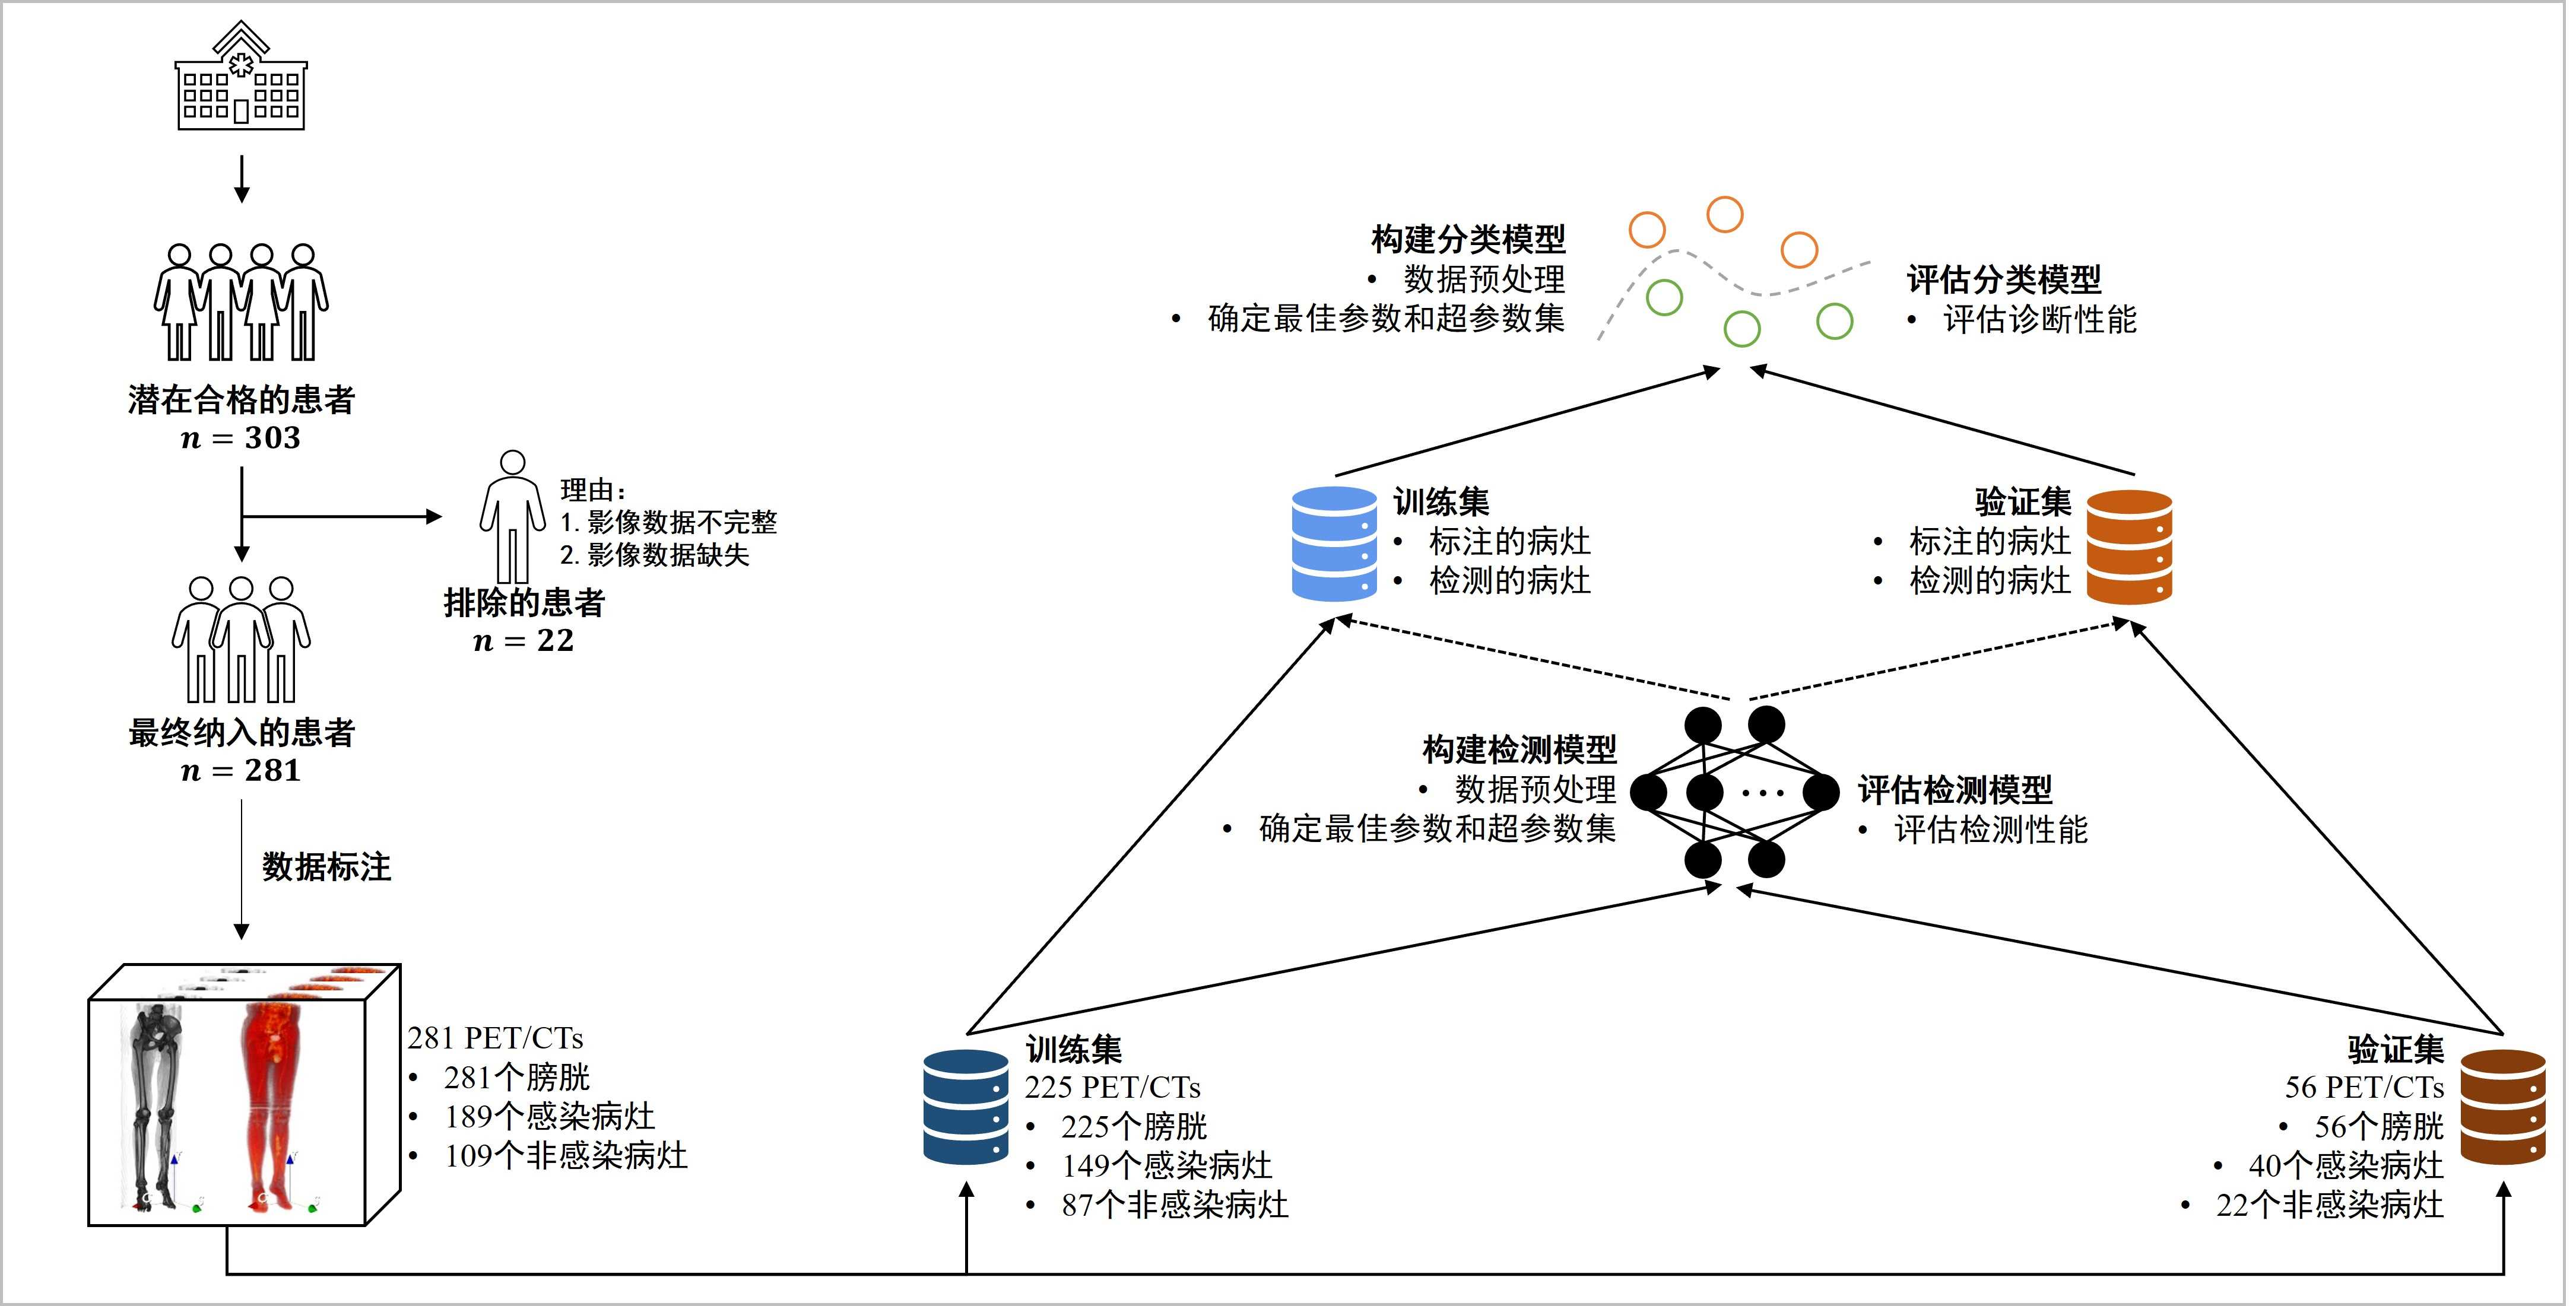
\includegraphics[width=\textwidth]{figures/chap04_study.jpg}
    \caption{本章研究的整体流程}
    \label{fig:chap04_study}
\end{figure}

本章研究的整体流程如图\ref{fig:chap04_study}所示。首先,通过最初的数据收集、筛选与标注,最终得到了包含了281名患者的PET/CT影像数据。其中,有281个膀胱标注、180个感染病灶标注和109个非感染病灶标注。其次,按照4:1的患者个体数量比例进行划分,得到了包含了225个患者PETCT影像数据的训练集(膀胱、感染病灶与非感染病灶:225 vs. 149 vs. 87)和包含了56个患者PETCT影像数据的验证集(膀胱、感染病灶与非感染病灶:56 vs. 40 vs. 22)。随后,设计和构建第一阶段的检测模型。通过使用训练集的训练结果,适应性地调整模型结构、超参数和训练策略,并利用验证集来进一步评估该模型的检测性能,获得最终的检测模型和最佳超参数。最后,设计和构建第二阶段的分类模型。利用第一阶段中检测模型在训练集和验证集中的检测结果添加到第二阶段的训练集和验证集中来扩充数据集的规模。同样地使用训练集的训练结果来适应性地调整模型、超参数和训练策略,并利用验证集来进一步评估该模型的分类性能,获得最终的分类模型和最佳超参数。最终二阶段的框架包含了最佳的检测模型和最佳的分类模型组成。

\section{数据预处理}

针对PET/CT影像中骨折相关感染的检测诊断任务,本章提出了一套完整的PET/CT影像的预处理算法,其具体流程如下:

(1)数据清洗与标注:清洗收集的患者PET/CT影像数据并进行三维目标框及其类别标注;

(2)PET/CT的转换与配准:首先,将CT影像中的像素值转换为用于测量组织对X射线的衰减程度的亨氏单位(Hounsfield Unit,HU),并且将PET影像中的像素值转换为用于半量化分析生理代谢活动的标准摄取值(Standardized Uptake Value, SUV)。然后,由于PET与CT影像的采样分辨率不一致,因此通过配准将PET和CT影像在物理空间中的原点、体素间距、尺寸大小变成一致。

(3)人体区域保留:考虑到PET/CT影像中非人体区域所占空间较大,并且机床属于纯粹的无关干扰区域,因此可彻底剔除该部分以提高影像质量和解剖学解析度。

(4)数据增强:通过翻转、适应性修改的Mixup和RICAP(Random Image Cropping And Patching)增加PET/CT影像中的检测目标数量,并扩充数据集的规模。

\subsection{数据清洗与标注}

\begin{figure}[htbp]
    \centering
    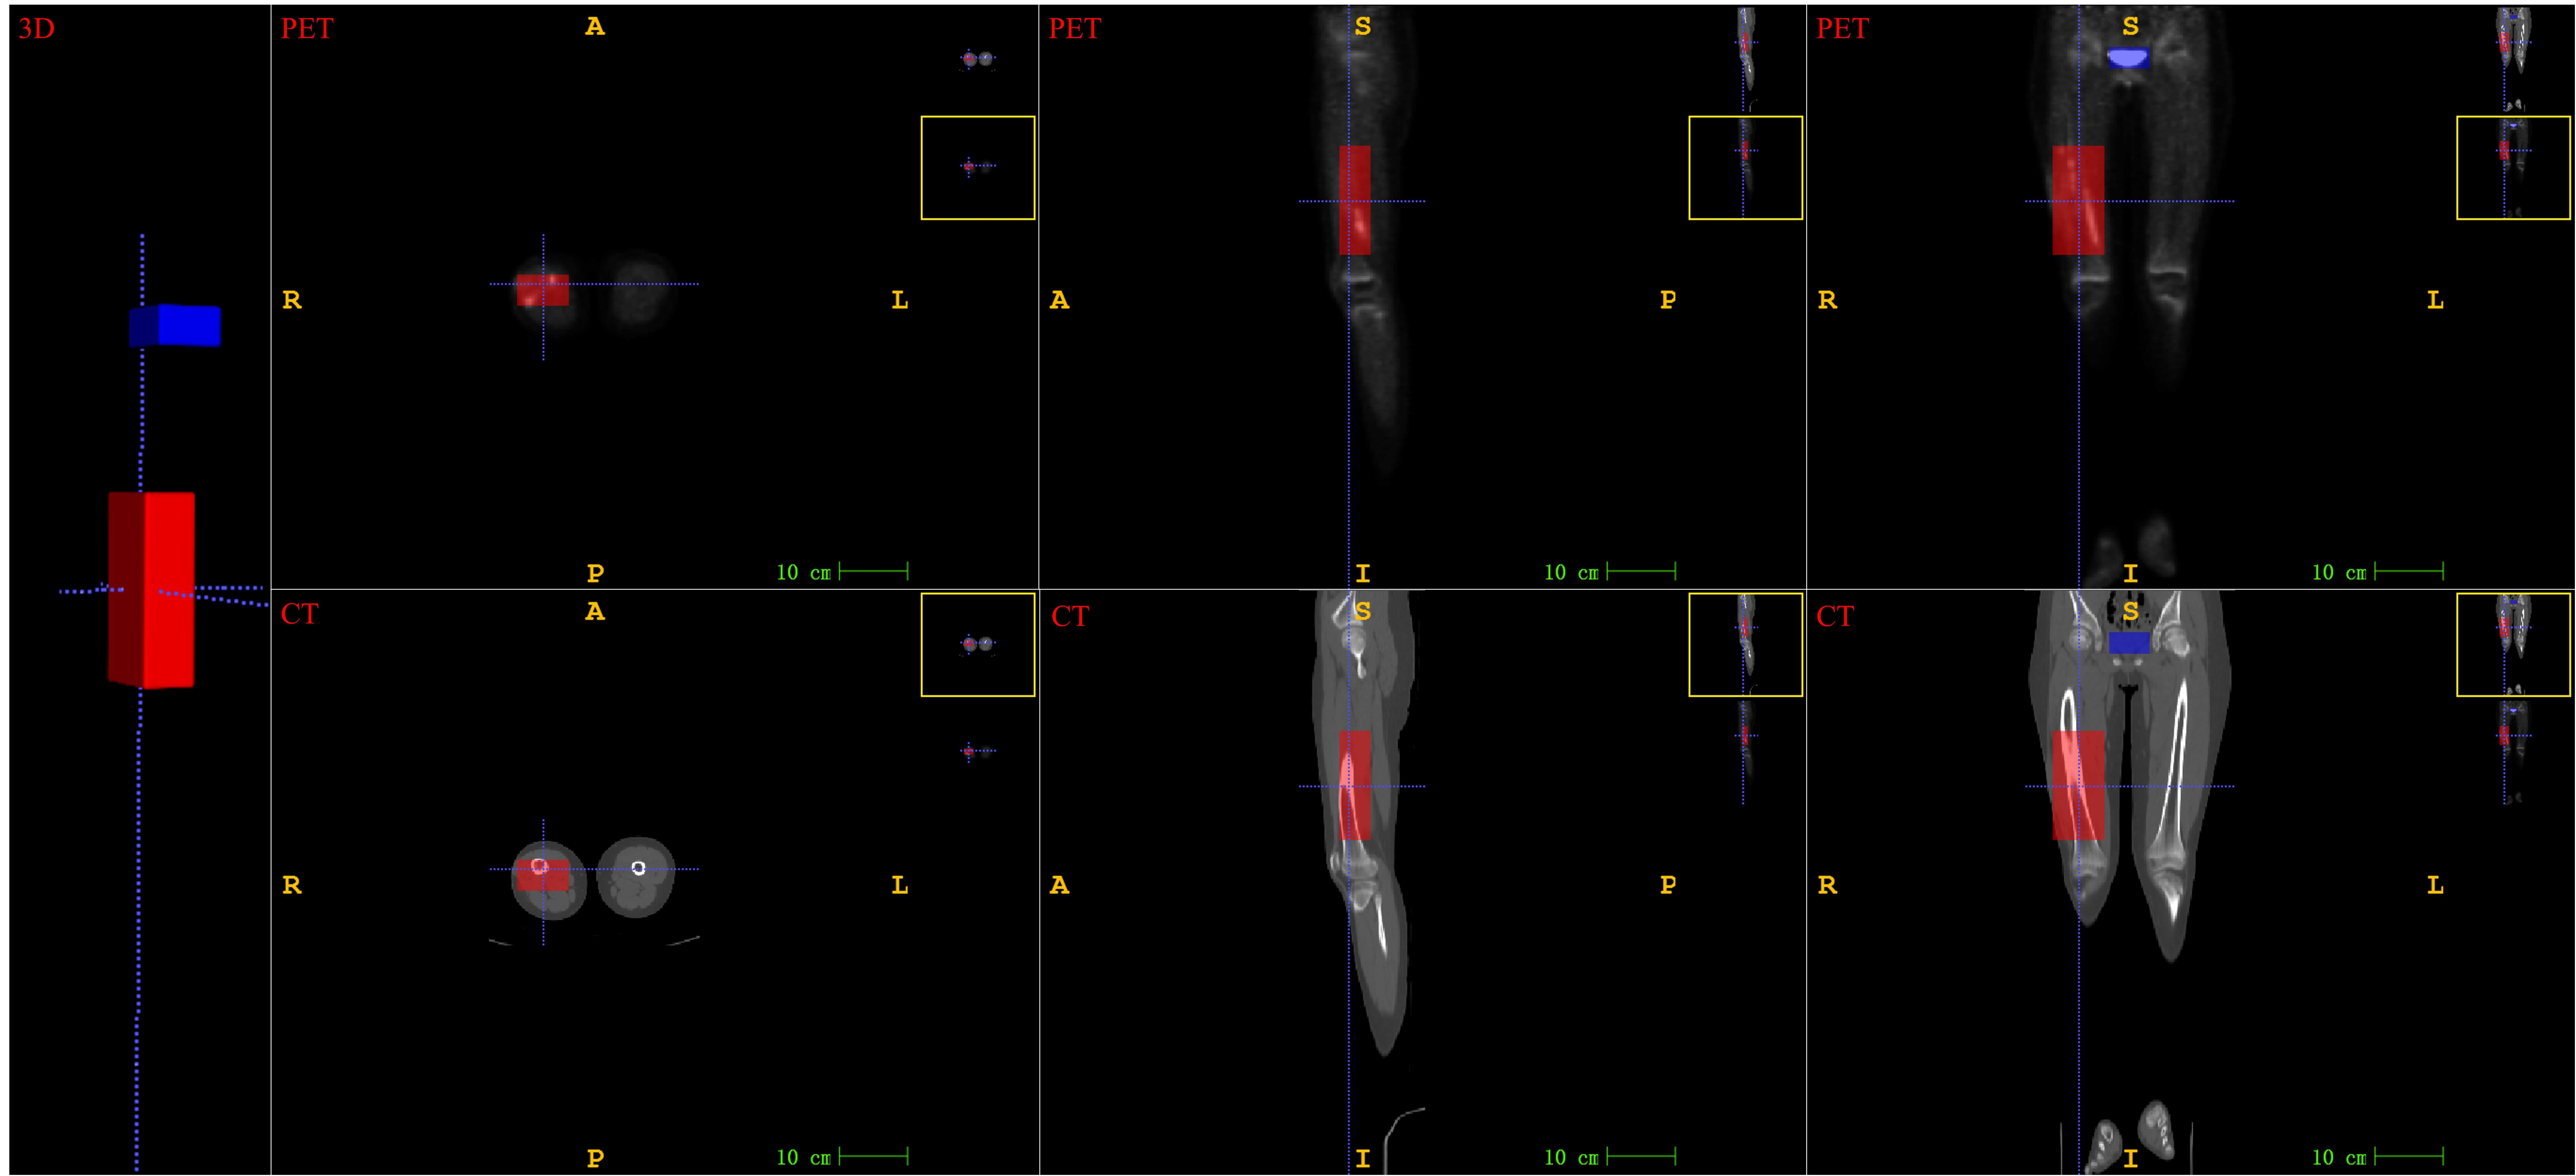
\includegraphics[width=\textwidth]{figures/chap04_label.jpg}
    \caption{PET/CT影像的数据标注}
    \label{fig:chap04_label}
\end{figure}

本章所采集的PET/CT影像数据同样是以DICOM格式存储。首先,对收集到的PET/CT影像数据进行清洗,例如排除掉不完整或存在缺失的影像数据。此外,为了保护病人的个人隐私信息,对DICOM格式文件进行脱敏,去除掉DICOM格式文件中有关于病人、医院、医生、设备制造商等等所有隐私数据。在经过上述操作后,本文作者在专业的核医学医生的指导下使用ITK-SNAP软件(v3.8.0, http://www.itksnap.org)对所有患者的PET/CT影像进行标注。最终标注结果由专业医学进行了核查。标注根据患者诊断报告为依据,在每一个患者的PET/CT影像上采用不同的颜色标注膀胱、感染病灶和非感染病灶,如图\ref{fig:chap04_label}所示。

\subsection{PET/CT的转换与配准}

HU是由CT扫描仪测量的组织相对于水的相对线性密度值。它提供了一种标定和对比度一致的方法,使得不同的CT扫描仪和不同扫描参数下的图像能够具有相似的密度值。此外,不同类型的组织对X射线具有不同的吸收能力,它们在CT中会展示出不同的亮度。将这些亮度转换为HU可以更加直观地表示组织的相对密度值,有助于区分不同的组织,也更方便于医生与研究人员进行更精确的定量分析。由此,本章将以DICOM格式存储的CT影像的像素值转换为HU值。

读取CT的DICOM文件,提取该文件中所需要的元数据:标签为(7FE0,0010)且关键字为像素数据(Pixel Data)的像素值\(P_{ct}\)、标签为(0028,1052)且关键字为重缩放截断值(Rescale Intercept)的截距\(b\)和标签为(0028,1053)且关键字为重缩放斜率(Rescale Slope)的斜率\(m\)。最后,通过公式\ref{eq:chap04_hu}转换为HU值。
\begin{equation}
    HU = m \times P_{ct} + b
    \label{eq:chap04_hu}
\end{equation}

SUV是一种用于衡量PET图像中肿瘤摄取的相对标准单位,通常用于定量分析和治疗反馈。SUV可以减少多种因素带来的影响,如患者的体重、注射剂量、扫描设备的差异、扫描时间、重建算法等等,使得不同患者、不同设备和不同扫描时期的PET影像结果具有可比性。此外,SUV值可以用于临床评估和治疗反馈,通过衡量肿瘤对放射性标记物的摄取程度,有助于评估肿瘤的活性、生物学特性以及治疗效果。由此,本文将以DICOM格式存储的PET影像的像素值转换为SUV值。

\begin{figure}[b]
    \centering
    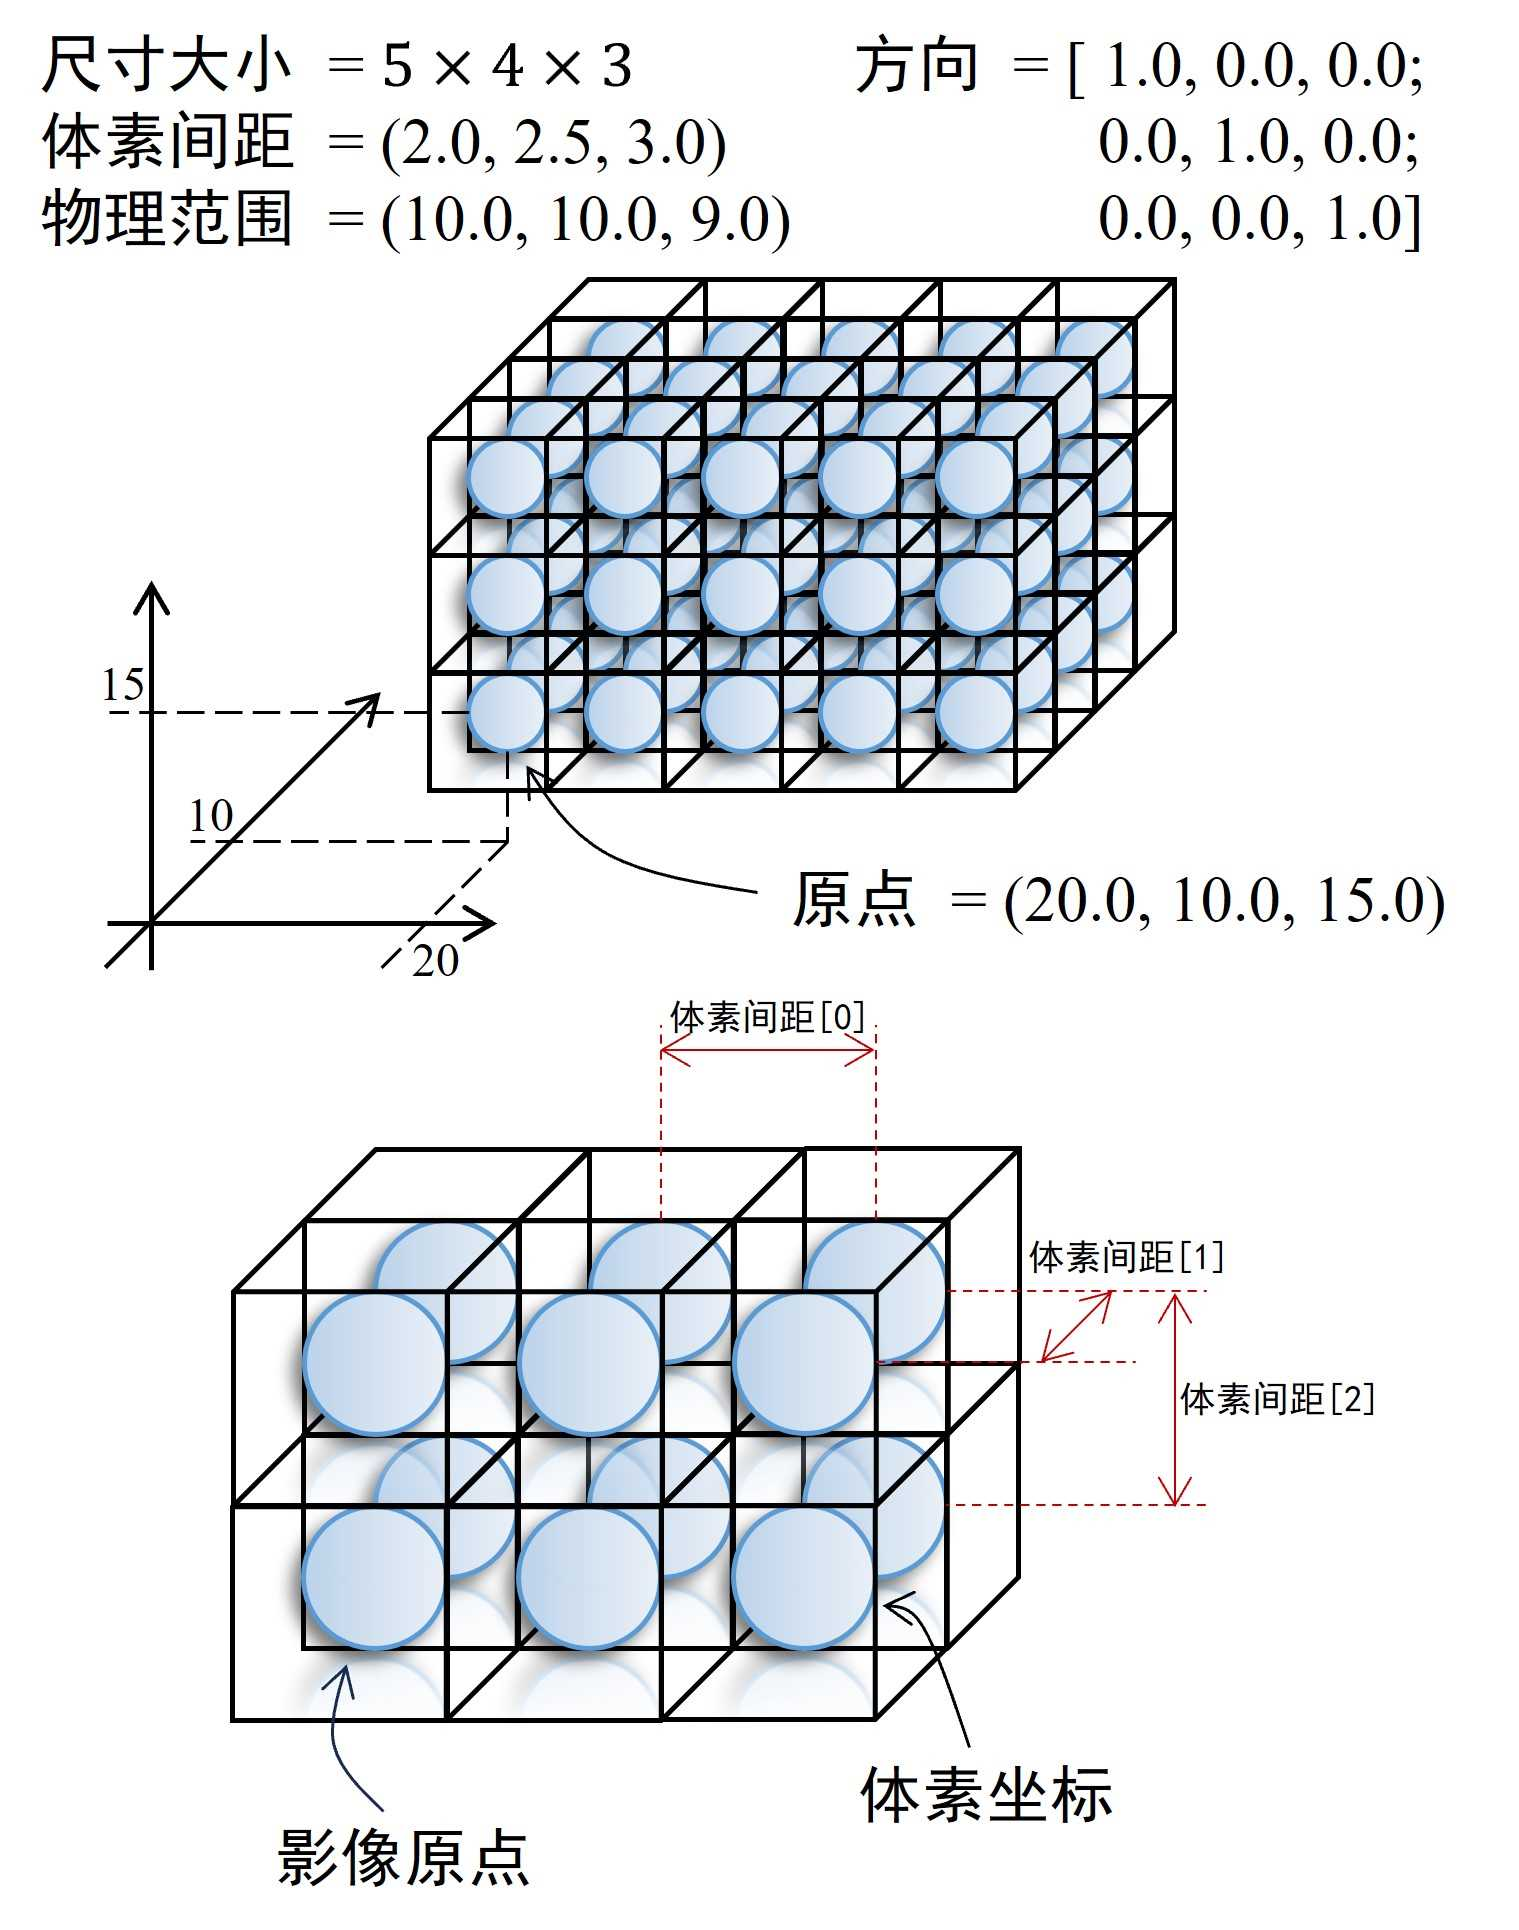
\includegraphics{figures/chap04_image.jpg}
    \caption{PET和CT影像在物理空间中所占据的区域}
    \label{fig:chap04_image}
\end{figure}

读取PET的DICOM文件。首先提取标签为(0010,1030)且关键字为病人体重(Patient Weight)的体重\(w\),计算病人的体重指标\(\mathcal{BW}\):
\begin{equation}
    \mathcal{BW} = 1000 \times w
\end{equation}
其次,提取标签为(0008,0021)且关键字为系列日期(Series Date)的扫描日期\(s_d\)、标签为(0008,0031)且关键字为系列时间(Series Time)的扫描时间\(s_t\)和标签为(0018,1072)且关键字为放射性药物开始时间(Radiopharmaceutical Start Time)的测量时间\(m_t\),来计算扫描到测量之间经过的时间\(\mathcal{T}\):
\begin{equation}
    \mathcal{T} = seconds(s_ds_t - s_dm_t)
\end{equation}
其中,\(seconds(\cdot, \cdot)\)表示计算两个时间戳之间的秒数。然后,提取标签为(0018,1074)且关键字为放射性核素总剂量(Radionuclide Total Dose)的注射剂量\(d\)和标签为(0018,1075)且关键字为放射性核半衰期计量(Radionuclide Half Life)的半衰期\(f\),来计算药物活性\(\mathcal{AC}\):
\begin{equation}
    \mathcal{AC} = d \times 2^{-\frac{\mathcal{T}}{f}}
\end{equation}
最后,提取标签为(7FE0,0010)且关键字为像素数据(Pixel Data)的像素值\(P_{pt}\)、标签为(0028,1052)且关键字为重缩放截断值(Rescale Intercept)的截距\(b\)和标签为(0028,1053)且关键字为重缩放斜率(Rescale Slope)的斜率\(m\),通过公式\ref{eq:chap04_suv}转换为SUV值。
\begin{equation}
    SUV = (m \times P_{pt} + b) \times \mathcal{BW} \div \mathcal{AC}
    \label{eq:chap04_suv}
\end{equation}

PET和CT是核医学影像中常见的两种三维模态影像。它们由一组点组成,每个点占据了空间中一部分物理区域。这与其他作为数组的图像之间存在着很大的差异,例如其他图像的像素或体素的间距是各向同性的,并且没有图像位置在物理空间的概念。如图\ref{fig:chap04_image}所示,PET和CT影像所占据的物理空间区域由影像的原点、间距、尺寸和方向余弦矩阵所确定。其中,原点是在每一维上的索引均为0的体素在世界坐标系上的位置;间距是每个维度上体素之间的间距;尺寸是每一个维度上体素的数量;方向余弦矩阵是每个轴的方向。

在本章收集的数据集中,PET和CT的原点、体素间距与尺寸大小都存在差异。因此,为了充分利用与融合PET和CT两种模态影像数据,本章采用了SimpleITK工具库\cite{yaniv2018simpleitk}进行配准。在经过前面处理计算得到的HU和SUV替换掉原来的像素值的基础上,使用SimpleITK中的函数Resample按照CT的原点、体素间距与尺寸大小对PET进行重采样。

\subsection{人体区域保留}

在对PET和CT进行转换和配准之后,由于PET和CT图像中含有过多与任务无关的区域以及CT中存在的扫描设备机床容易影响模型训练和检测性能。本章提出了一个人体区域保留算法,人体区域保留前后效果如图\ref{fig:chap04_body_retent}所示。人体区域保留算法流程如下:

\begin{figure}[htbp]
    \centering
    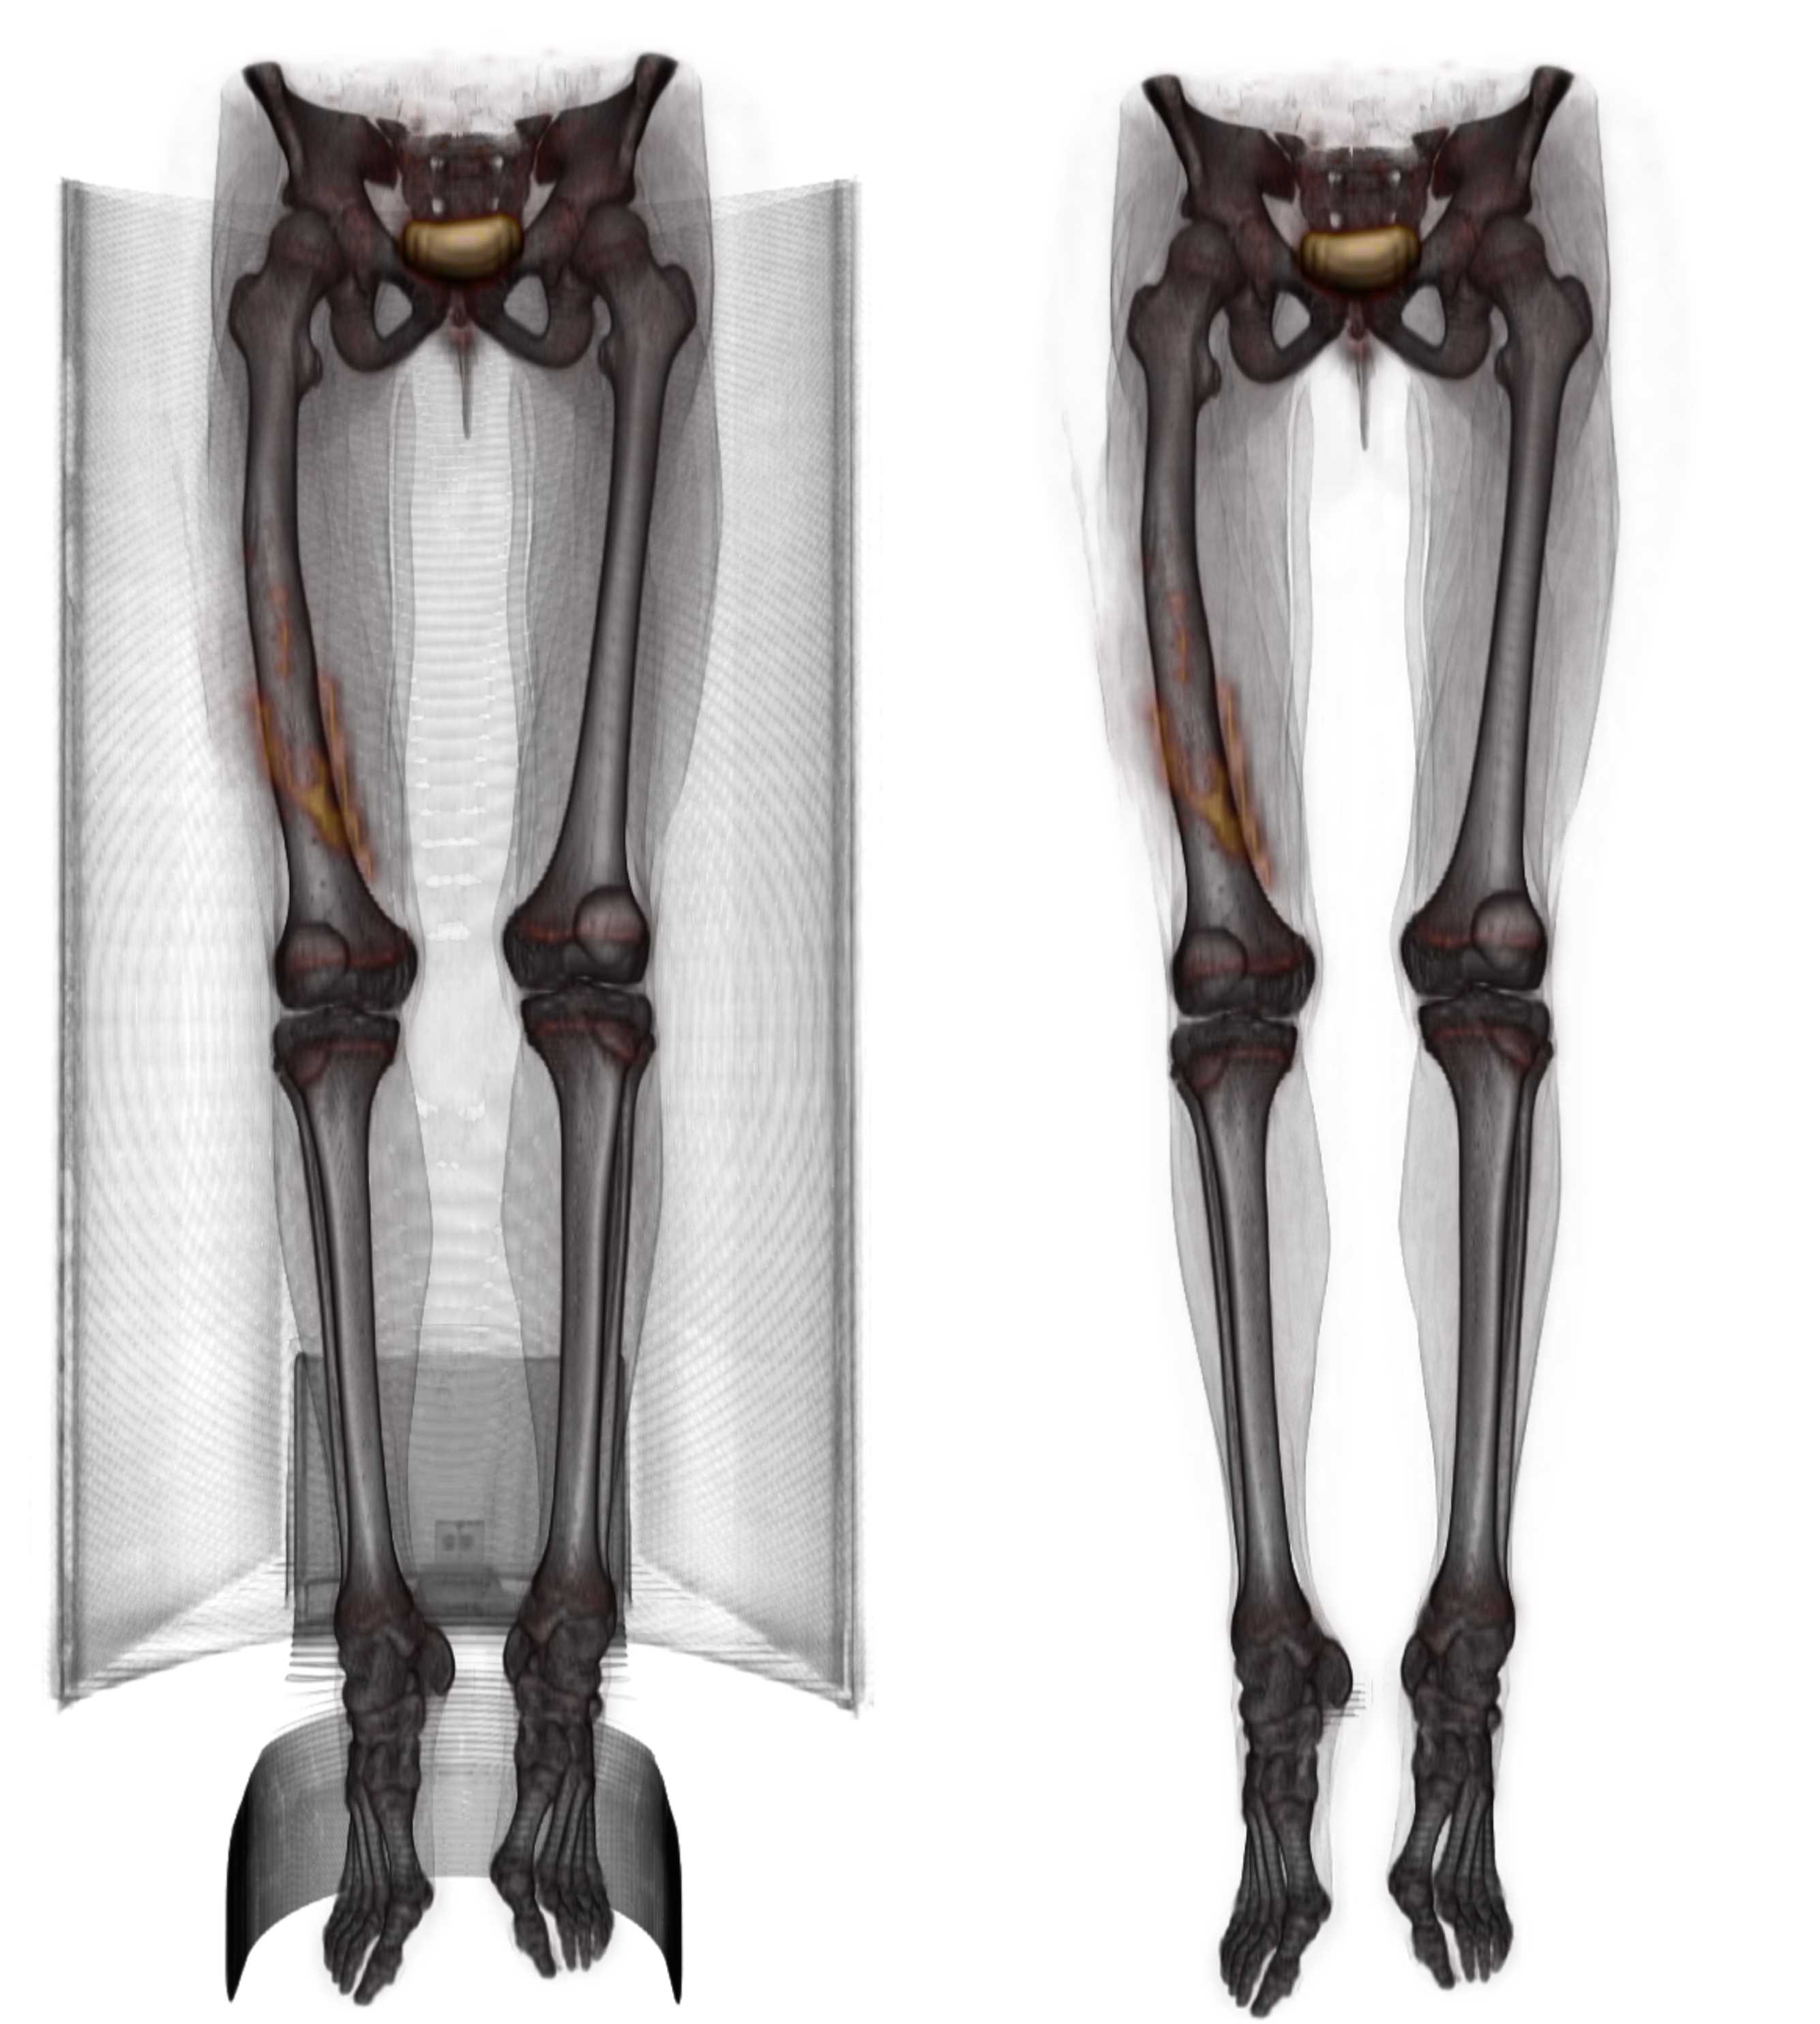
\includegraphics[width=0.8\textwidth]{figures/chap04_body_retent.png}
    \caption{人体区域保留算法前后对比}
    \label{fig:chap04_body_retent}
\end{figure}

(1)读取CT影像中的HU三维数组\(Arr_{HU}\)和PET影像中的SUV三维数组\(Arr_{SUV}\)。通过在CT和PET上分别进行图像二值化计算出初步的分割掩码图\(maskB_{HU}\)和\(maskB_{SUV}\),如公式\ref{eq:chap04_mask_binary}所示:
\begin{equation}
    \begin{aligned}
        maskB_{HU}^{i, j, k}  & =
        \begin{cases}
            1 , & \text{if \(Arr_{HU}^{i, j, k} > -200\)} \\
            0 , & \text{otherwise}
        \end{cases}  \\
        maskB_{SUV}^{i, j, k} & =
        \begin{cases}
            1 , & \text{if \(Arr_{SUV}^{i, j, k} > 0.001\)} \\
            0 , & \text{otherwise}
        \end{cases} \\
    \end{aligned}
    \label{eq:chap04_mask_binary}
\end{equation}
其中,\(i,j,k\)表示三个维度上的索引。

(2)使用一个核半径为2且形态为球形的图像滤波\(F_2\)对二值化得到的分割掩码图进行形态学闭操作,用以去除小孔,平滑边界,使得分割掩码图更加完整,如公式\ref{eq:chap04_mask_close}所示:
\begin{equation}
    \begin{aligned}
        maskB_{HU}  & = (maskB_{HU} \oplus F_2 ) \ominus F_2  \\
        maskB_{SUV} & = (maskB_{SUV} \oplus F_2 ) \ominus F_2
    \end{aligned}
    \label{eq:chap04_mask_close}
\end{equation}
其中,\(\oplus\)表示形态学上的膨胀操作,\(\ominus\)表示形态学上的腐蚀操作。

(3)计算分割掩码图\(maskB_{HU}\)和\(maskB_{SUV}\)的最大连通量。首先,扫描分割掩码图,对其中的每个连通区域标记一个唯一的标签\(L\)。然后,统计每一个标记区域的体素数量\(S\)。最后,选择具有最大体素数量的标记区域,即最大连通量:
\begin{equation}
    L_{max} = \mathop{\arg\max}_{i=1}^N S_i
\end{equation}
其中,\(N\)表示标签的总数,\(S_i\)表示标签为\(i\)的区域的体素数量。再计算仅保留最大连通量的分割掩码图并计算出它们两的交集:
\begin{equation}
    \begin{aligned}
        mask_{HU}^{i,j,k}  & =
        \begin{cases}
            1, & \text{if \(maskB_{HU, max}^{i,j,k} = L_{HU,max}\)} \\
            0, & \text{otherwise}
        \end{cases}  \\
        mask_{SUV}^{i,j,k} & =
        \begin{cases}
            1, & \text{if \(maskB_{SUV, max}^{i,j,k} = L_{SUV,max}\)} \\
            0, & \text{otherwise}
        \end{cases} \\
        mask               & = mask_{HU} \cap mask_{SUV}
    \end{aligned}
\end{equation}
其中,\(maskB_{HU, max}\)和\(maskB_{SUV, max}\)为计算最大连通量时对每个连通区域标记了唯一标签的三维数组。\(L_{HU,max}\)和\(L_{SUV,max}\)分别是\(maskB_{HU, max}\)和\(maskB_{SUV, max}\)的最大连通量的标签。

(4)使用一个核半径为20且形态为球形的图像滤波\(F_{20}\)对最后的分割掩码图\(mask\)进行形态学闭操作,去除伪影,使得分割掩码图更加完整,得到最终的人体区域掩码图\(mask_{body}\)。
\begin{equation}
    mask_{body} = (mask \oplus F_{20} ) \ominus F_{20}
\end{equation}

(5)根据\(mask_{body}\)计算出可以包围人体区域的最小立方体,对CT、PET和\(mask_{body}\)进行裁剪。最后,根据\(mask_{body}\)将属于非人体区域中的CT的HU值设为-1000,PET的SUV值设为0,如公式\ref{eq:chap04_crop_resign}所示。
\begin{equation}
    \begin{aligned}
        Arr_{HU}^{i, j, k}  & = -1000 \quad & \text{where \(mask_{body}^{i,j,k} = 0\)} \\
        Arr_{SUV}^{i, j, k} & = 0 \quad     & \text{where \(mask_{body}^{i,j,k} = 0\)}
    \end{aligned}
    \label{eq:chap04_crop_resign}
\end{equation}

\subsection{数据增强}

由于骨折相关感染的PET/CT数据集规模较小、检测目标数量少,导致在一定程度上增加了模型的训练难度。对于这种小规模和少样本的情况可能影响到模型对于骨折相关感染的全面理解和准确检测的问题,本章研究需要采用有效的数据增强方法以提高模型的泛化性能,并使其更好地适应不同类型的病灶区域。因此,本章提出了三种数据增强的方法,如图\ref{fig:chap04_augmentation}所示,分别是镜像翻转、适应性修改的Mixup和RICAP。

\begin{figure}
    \centering
    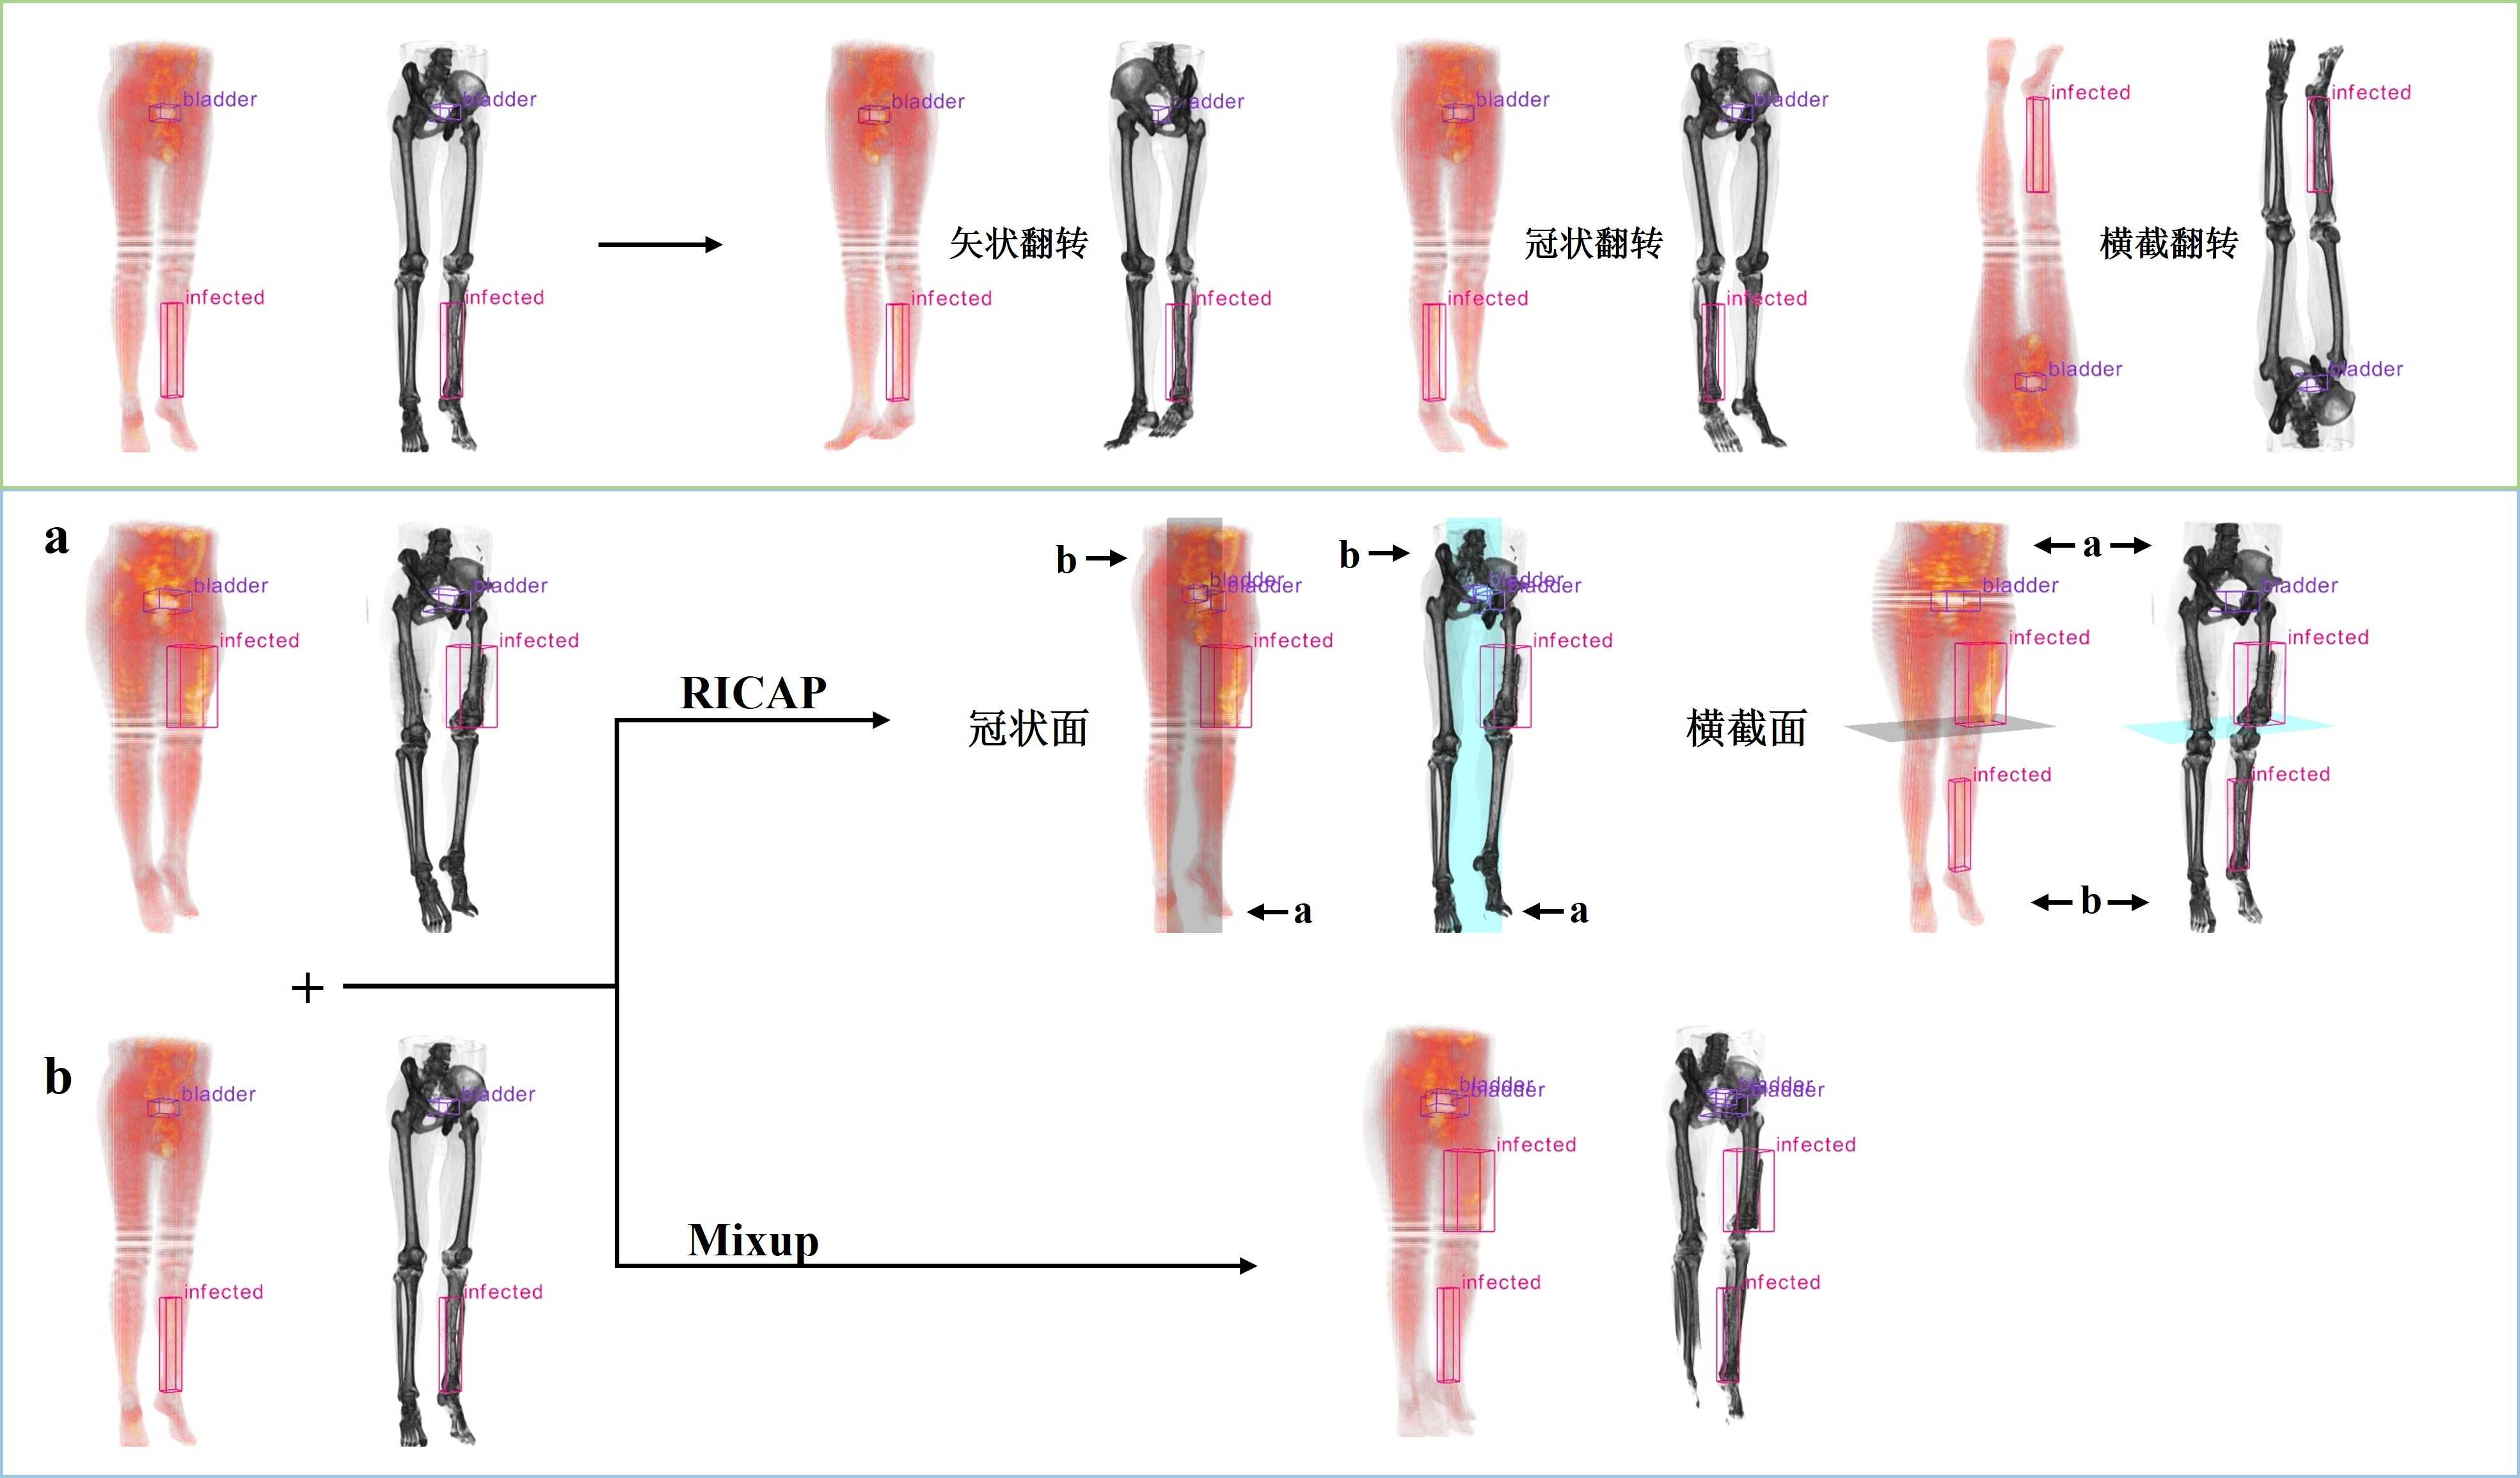
\includegraphics[height=\textwidth, width=0.95\textheight,angle=90,keepaspectratio]{figures/chap04_augmentation.jpg}
    \caption{应用于PET/CT影像上的数据增强方法}
    \label{fig:chap04_augmentation}
\end{figure}

翻转属于单样本的数据增强方法,对单个样本随机地在矢状轴、管状轴和横断轴中一个方向上翻转。而Mixup和RICAP则是属于多样本的数据增强方法,通过各自地方法使用两个样本去合成一个新的样本。

Mixup的基本原理是通过对多个输入样本及其标签进行相同比例的混合,从而生成新的输入样本和标签。由此,在本章研究中,为了将原用于分类任务中的Mixup应用于目标检测任务,Mixup数据增强方法进行了适应性地修改。对于两个输入样本\(image_1\)和\(image_2\)以及它们的标签\(box_1\)和\(box_2\),输入样本进行等比例的混合生成新的输入样本\(image_{new}\),而标签采用并集的方式合成新的标签\(box_{new}\),如公式\ref{eq:chap04_mixup}所示:
\begin{equation}
    \begin{aligned}
        image_{new} & = 0.5 \times image_1 + 0.5 \times image_2 \\
        box_{new}   & = box_1 \cup box_2
    \end{aligned}
    \label{eq:chap04_mixup}
\end{equation}

RICAP的基本原理是通过多个输入样本按照不同的所占区域下进行裁剪,裁剪得到的样本按照所占区域的相对位置进行拼接生成新的输入样本,而标签则按照它们输入样本所占区域占新样本总体区域的大小为比例进行混合生成新标签。由此,在本章研究中,同样适用于分类任务中的RICAP进行了适应性地修改,以更加适合于骨折相关感染病灶检测任务。首先,随机地在矢状轴和横断轴方向上二选一。随后,在选中的方向上随机地选择需要裁剪的区域。最后,根据裁剪区域的相对位置拼接裁剪下来的输入样本生成新的输入样本。裁剪区域的计算方式如下:

假设输入样本的大小为\((W,H,D)\)。如果在矢状轴上进行裁剪与拼接,则对于两个输入样本的裁剪区域分别为\((1, 1, 1)\thicksim (\omega, H, D)\)和\((\omega + 1, 1, 1)\thicksim (W, H, D)\)。如果在横断轴上进行裁剪,则对于两个输入样本的裁剪区域分别为\((1, 1, 1)\thicksim (W, H, \delta)\)和\((1, 1, \delta + 1)\thicksim (W, H, D)\)。其中,\(\omega\)和\(\delta\)的计算方式如\ref{eq:chap04_ricap}所示。
\begin{equation}
    \begin{aligned}
        \omega & = round(\omega) & \quad \omega & \sim U(0.4\times W, 0.6 \times W) \\
        \delta & = round(\delta) & \quad \delta & \sim U(0.4\times D, 0.6 \times D) \\
    \end{aligned}
    \label{eq:chap04_ricap}
\end{equation}
其中,\(round(\cdot)\)表示取整函数,\(X \sim U(a, b)\)表示\(X\)服从区间\((a,b)\)上的均匀分布。

\section{框架设计}

\begin{figure}
    \centering
    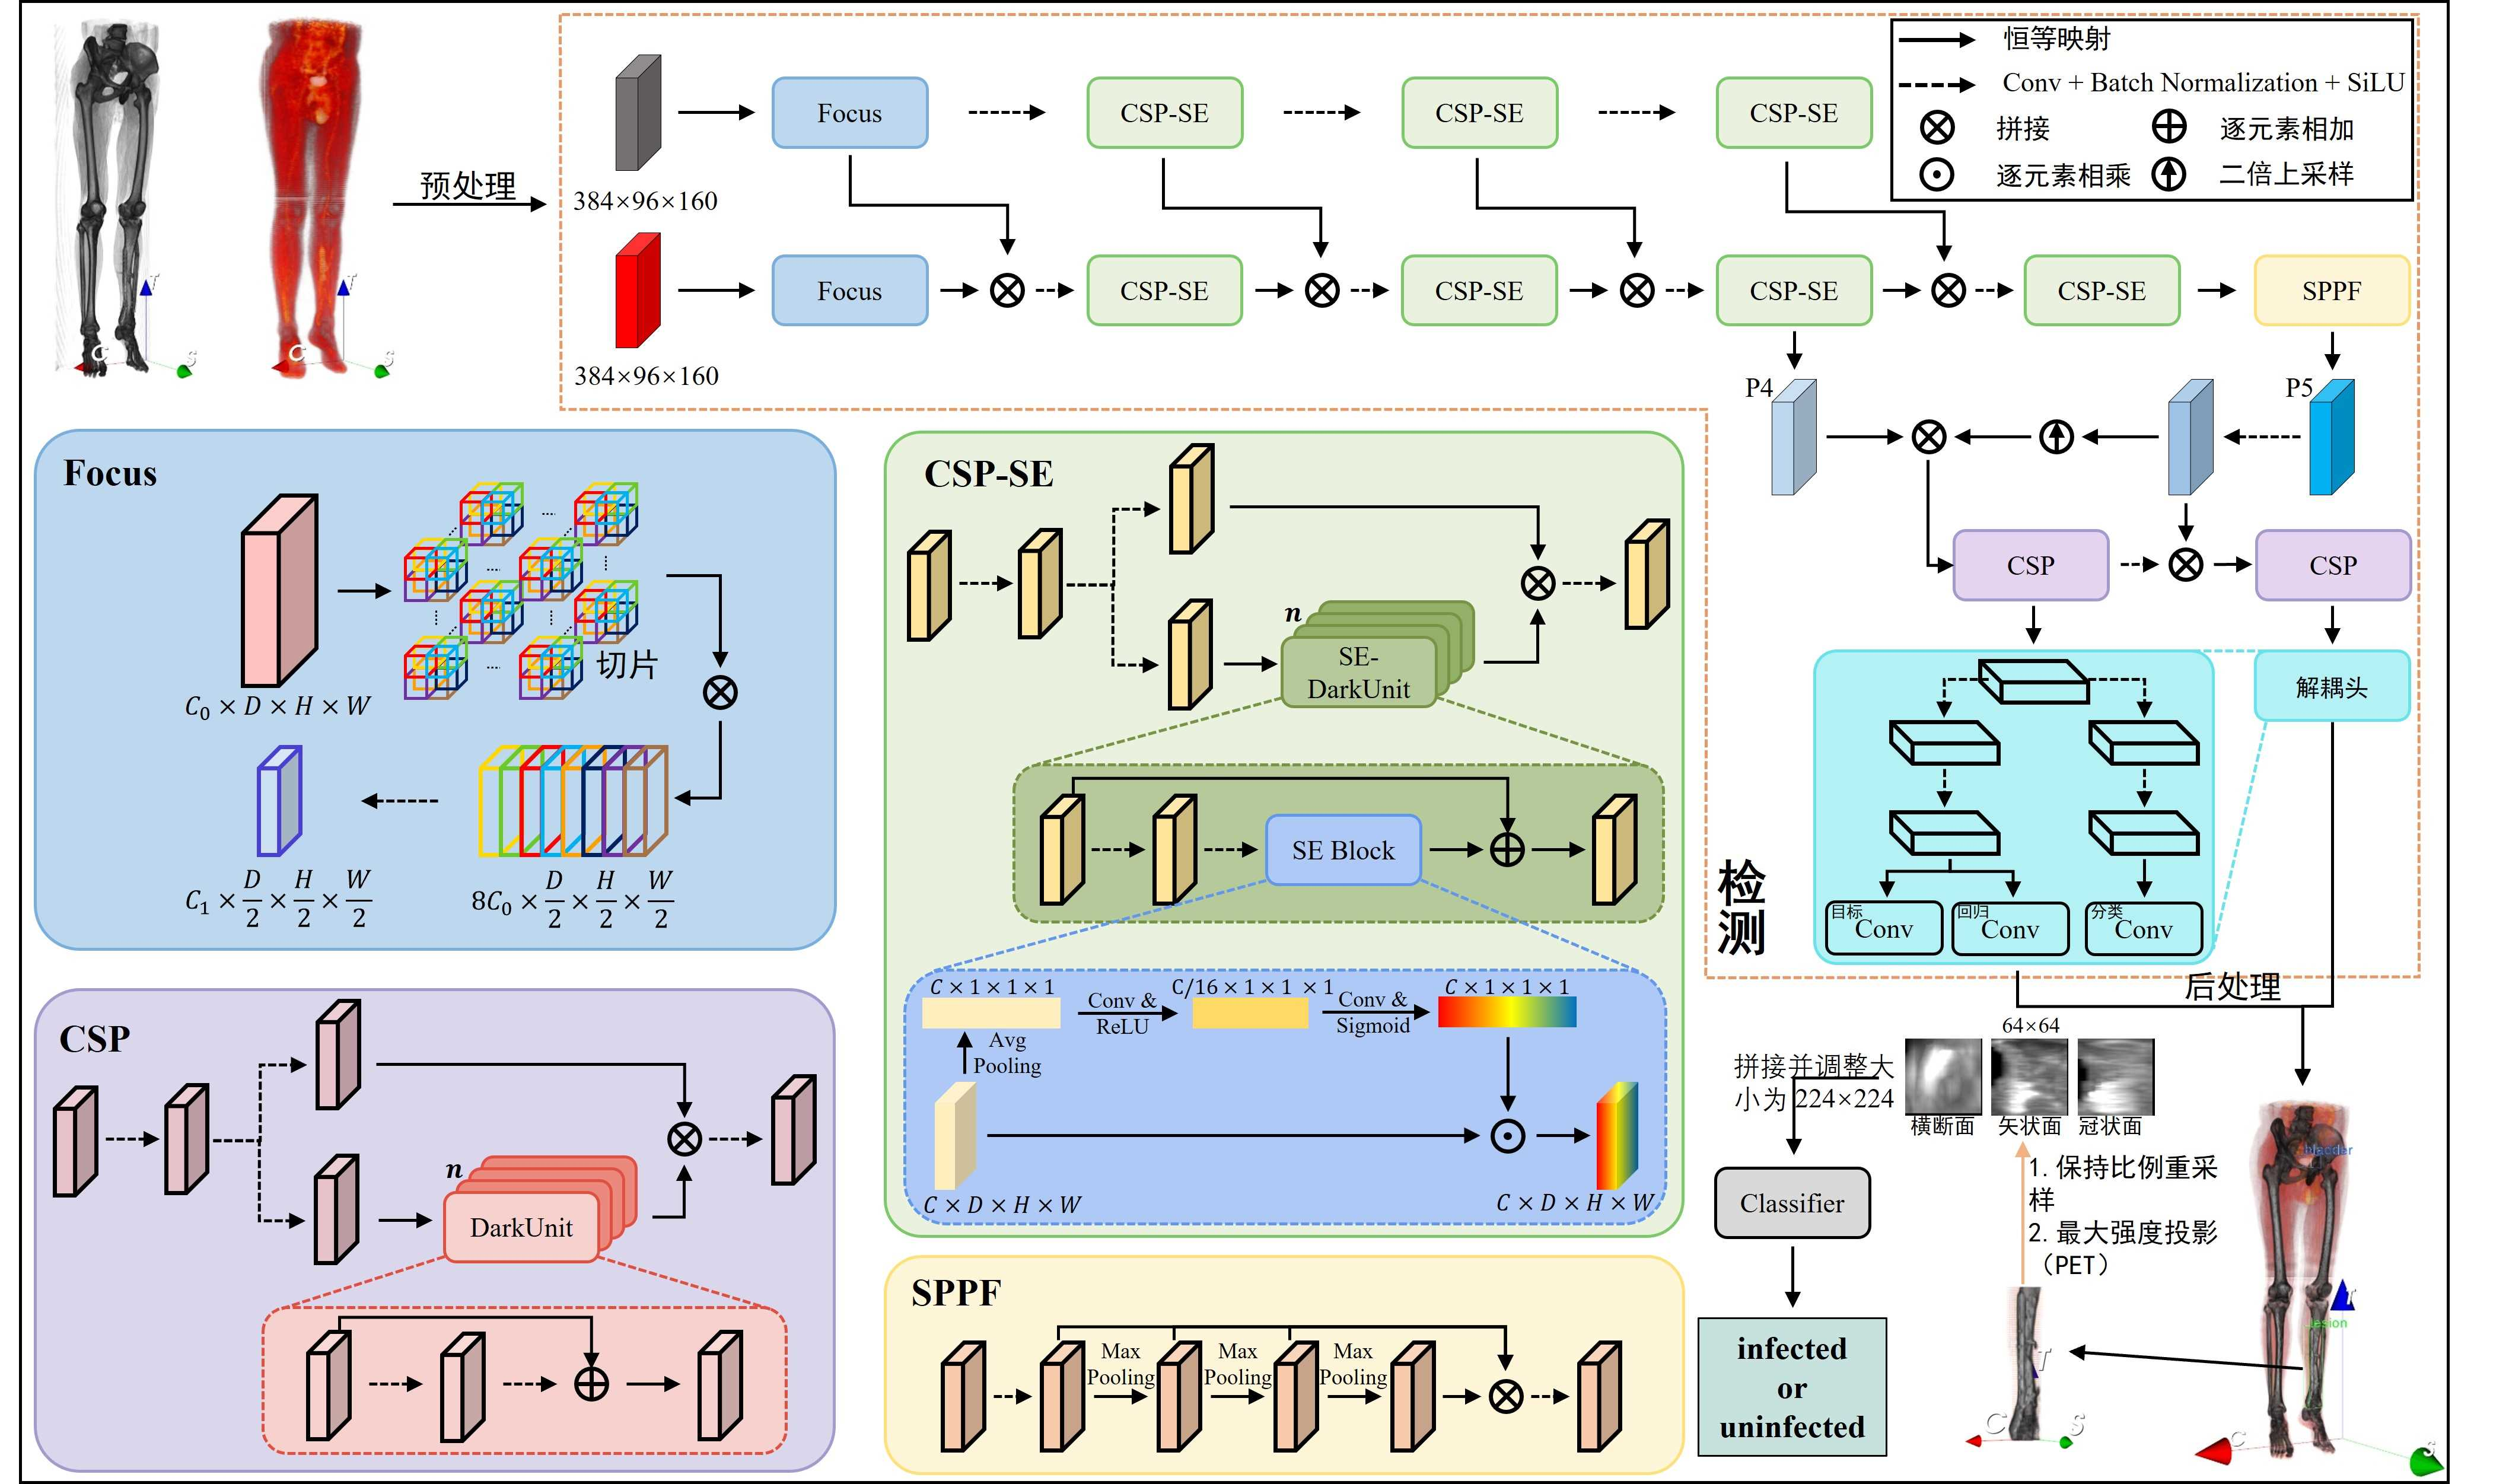
\includegraphics[width=0.95\textheight,height=\textwidth,angle=90,keepaspectratio]{figures/chap04_model.jpg}
    \caption{两阶段的病灶检测诊断分类网络框架示意图}
    \label{fig:chap04_model}
\end{figure}

PET/CT影像是两种模态组合的三维影像数据,它们展示了一个患者在注射药剂后的解剖组织信息和生理代谢信息。针对PET与CT影像之间存在互补互助的特性。本章在骨折相关感染的诊断方法中设计了一个两阶段的病灶检测诊断分类网络框架3DFRINet,整体架构如图\ref{fig:chap04_model}所示。整个网络框架分为病灶检测网络与病灶诊断分类网络,采用先检测后分类的两阶段网络框架的设计,可以排除掉与病灶无关的大部分区域,使得病灶诊断分类网络更加关注于病灶区域的生理代谢信息。病灶检测网络322-YOLO(3 dimensions 2 paths 2 heads YOLO)通过双分支设计和注意力模块,进一步优化对骨折相关感染病灶的定位。按照YOLO的结构设计也提高网络对于小尺度和多尺度病灶的检测精度,同时有效地减少了错检率。病灶诊断分类网络对候选区域进一步挖掘病灶的代谢形态特征,实现对骨折相关感染的准确分类。

\subsection{病灶检测网络322-YOLO}

经过本章引入的预处理流程后,将PET和CT影像数据重采样至\(384 \times 96\times 160\),并将CT的HU以300为窗位,1500为窗宽进行归一化,PET的SUV中小于0的统一为0。随后,被输入到322-YOLO病灶检测网络,对骨折相关感染病灶区域进行检测和识别。322-YOLO在YOLOX\cite{ge2021yolox}的基础上改进而来,由用于特征提取的双分支主干网络,整合两个不同层次下的特征图的颈部网络以及用于预测目标的种类、大小和位置的头部网络组成。

双分支主干网络可以分为PET主分支和CT辅助分支,当PET主分支持续提取生理代谢信息特征的同时,来自于CT辅助分支的解剖信息特征也被逐阶段地融入生理代谢信息特征之中。PET主分支主要由Focus、CSP-SE和SPPF模块构成,而CT辅助分支主要由Focus和CSP-SE模块构成。Focus模块从三个维度上以一个体素间隔对输入数据进行切片,随后拼接切片得到的8个子块,然后通过卷积进行特征提取与下采样。它将PET中的生理信息和CT中的解剖信息从空间维度堆叠到通道维度,在不牺牲特征信息的前提下,提高卷积操作对生理和解剖信息的感知范围,为网络提供了更广泛的上下文信息,有助于准确定位和识别感染病灶。CSP-SE模块(the Cross Stage Partial-Squeeze and Excitation dark unit)在dark unit的基础上结合了跨阶段部分结构\cite{wang2020cspnet}和通道注意力模块\cite{hu2018squeeze}。跨阶段部分结构允许特征在不同层之间进行更有效的信息传递和融合,有助于捕捉不同尺度和抽象级别的特征。同时,通道注意力模块的引入使得CSP-SE模块能够根据特定通道的重要性调整特征的权重,进一步提升网络对骨折相关感染病灶的关注度。通过充分结合了多层次的特征表达和通道级的信息调控,为网络在处理骨折相关感染特征上提供了更为丰富和精准的上下文信息。SPPF模块是由SPP\cite{he2015spatial}改进而来,具有更少的参数,更快的计算速度。它可以整合不同尺度的特征,以更好地适应骨折相关感染病灶的多样性(例如病灶区域大小、生理代谢或解剖结构上的差异),减轻对单一尺度特征的过度依赖,全面地捕捉病灶区域的上下文信息。

用于训练模型的输入样本为\(\text{SUV}, \text{HU} \in R^{C \times D \times H \times W}\),其中\(C,D,H,W\)分为是输入样本的通道数、深度、高度和宽度。由于正负样本存在极度不平衡的问题,因此病灶检测网络不再使用最大的同时也是正负样本最不平衡的特征图\(P_3\)。则由双分支主干网络提取的两个尺度下的特征图\(P_4\)和\(P_5\)的计算方式如\ref{eq:chap04_backbone}所示。
\begin{equation}
    \begin{aligned}
        P_1^{HU}  & = \text{Focus}(HU) \quad P_1^{SUV} = \text{Focus}(SUV)         \\
        P_i^{HU}  & = \text{CSP-SE}(\text{CBS}(P^{HU}_{i-1}))                      \\
        P_j^{SUV} & = \text{CSP-SE}(\text{CBS}(P^{HU}_{j-1} \oplus P^{SUV}_{j-1})) \\
        P_4       & = P_4^{SUV} \quad P_5 = \text{SPPF}(P_5^{SUV})
    \end{aligned}
    \label{eq:chap04_backbone}
\end{equation}
其中,\(P_i^{HU}(i=2,3,4)\)表示为第\(i\)阶段中CT辅助分支提取的特征图,\(P_j^{SUV}(j=2,3,4,5)\)表示为第\(j\)阶段中PET主分支融合并提取的特征图,CBS表示一个由卷积、批归一化和SiLU构成的基础模块,\(\oplus\)表示拼接操作。

颈部网络的结构由自顶向下和自底向上两条路径组成,以融合不同层次下的特征图,来提高对病灶的准确定位和识别。自顶向下的路径通过将丰富的语义信息(例如目标的类别信息)传播到浅层特征图,为网络提供更高层次的语义理解。与此同时,自底向上的路径则将目标的位置和大小信息传递到深层特征图,使得不同层次的特征在融合后既包含丰富的目标类别特征,又包含位置和大小信息。这种双向信息传递的机制有助于更全面地捕捉感染病变的特征,从而提高检测准确性。与此同时,自底向上的路径聚合了所有特征层的路径,从而缩短了底层与顶层特征之间的距离。这样的结构有助于更快地传播底层特征到上层,提高了网络对于病灶不同层次特征的有效利用,增强了整体网络的表达能力。通过自顶向下的路径计算得到\(P_4^{neck}\)和自底向上的路径计算得到\(P_5^{neck}\),如\ref{eq:chap04_neck}所示。
\begin{equation}
    \begin{aligned}
        P_4^{neck} & = \text{CSP}(\text{Upsample}(\text{CBS}(P_5)) \oplus P_4)    \\
        P_5^{neck} & =  \text{CSP}(\text{CBS}(P_5) \oplus \text{CBS}(P_4^{neck}))
    \end{aligned}
    \label{eq:chap04_neck}
\end{equation}
其中,Upsample表示2倍上采样。

头部网络采用解耦的模式,通过在颈部网络融合的特征中独立地进行目标的类别、位置和大小的预测,有效减少了不同预测任务之间的互相干扰。这种解耦设计使得模型可以更准确地预测定位目标的类别,同时在空间上准确定位病灶的位置和大小,从而提高了整体检测性能。其计算方式如\ref{eq:chap04_head}所示。
\begin{equation}
    \begin{aligned}
        P_c   & = \text{CBS}(\text{CBS}(P_n^{neck})) \\
        cls_n & = Conv_1(P_c)                        \\
        P_r   & = \text{CBS}(\text{CBS}(P_n^{neck})) \\
        reg_n & = Conv_2(P_r)                        \\
        obj_n & = Conv_3(P_r)                        \\
    \end{aligned}
    \label{eq:chap04_head}
\end{equation}



(1)无先验框

322-YOLO跟YOLOX一致,采用了无先验框的方式,但在YOLOX的基础上添加了需要预测的值。在解耦头中,独立预测的目标类别设置为2类,分别是病灶和膀胱;目标大小从4个值改成了6个值,即预测框在三维网格中位于左上后方的三个偏移量以及预测框的宽、高和深。在检测网络最终预测的不同层次下的特征图中,根据目标的中心位置以及预定义的范围去分配相应的正样本。

(2)分配策略

322-YOLO跟YOLOX在正样本分配策略上的一致,作为一个无先验框的目标检测方法,对每一个目标不仅仅只分配一个位于中心位置的正样本,同时还关注其他高质量的预测。通过关注这些高质量的预测也可能带来有益的梯度,这从一定程度上来说可以缓解训练过程中正负样本的极端不平衡。简单地来说,322-YOLO通过将以目标的中心位置为中心点,以2.5为半径的正方体区域设置为正样本,同时也将目标框中的区域设置为正样本。这中正样本分配方式一定程度上可以提升目标检测器的检测性能。

在目标检测任务中,标签分配策略也是很重要的一部分。SimOTA是OTA(Optimal Transport Assignment)\cite{ge2021ota}的一种简化近似版本。OTA是从一个全局视角中去分析标签分配的方式并将分配过程表述为最优传输问题(Optimal Transport)。通过免去手工选定参数的方式,使得真实框匹配多个更加合适的多个预测框。SimOTA将OTA的优化过程简化为动态top-k策略。首先,计算每个真实框与预测框之间的成对匹配度\(c\),通过使用预测框\(p_n\)与真实框\(g_m\)损失来表示,如公式:
\begin{equation}
    c_{mn} = L^{cls}_{mn} + \lambda L^{reg}_{mn}
\end{equation}
其中,\(\lambda\)表示平衡系数,\(L^{cls}_{mn}\)和\(L^{reg}_{mn}\)是真实框\(g_m\)与预测框\(p_n\)之间的分类损失和回归损失。对于每个真实框,进一步地在满足前面所述的正样本分配策略的基础上,选择具有前k个最小的成对匹配度的预测框。其中,成对匹配度越低表示真实框与预测框越合适。最终,将这些满足条件的预测框所在特征图的网格位置设置为正样本,其他的网格设置为负样本。

(3)损失函数

通过SimOTA标签分配策略对每个目标都分配相应的正负样本之后,二元交叉熵损失函数(Binary Cross Entropy Loss)用于计算区分正负样本的损失\(\mathcal{L}_{obj}\)和目标类别的损失\(\mathcal{L}_{cls}\),交并比损失函数(IoU Loss)用于计算目标尺寸大小的损失\(\mathcal{L}_{reg}\)。对于预测框\(p = (p^{obj}, p^{cls}, p^{reg})\)和真实框\(g = (g^{obj}, g^{cls}, g^{reg})\),三种损失的计算方式如\ref{eq:chap04_loss1}所示。
\begin{equation}
    \begin{aligned}
        \mathcal{L}_{obj} & = -\sum_{i=0}^I( g^{obj}_{bi} \log p^{obj}_{bi} +  (1- g^{obj}_{bi})\log(1-p^{obj}_{bi} ))      \\
        \mathcal{L}_{cls} & = -\sum_{k=0}^K( g^{cls}_{bk} \log p^{cls}_{bk} +  (1- g^{cls}_{bk})\log(1-p^{cls}_{bk} ))      \\
        \mathcal{L}_{reg} & = \sum_{k=0}^K( 1 - (\frac{g^{reg}_{bk} \cap p^{reg}_{bk}}{g^{reg}_{bk} \cup p^{reg}_{bk}})^2 ) \\
    \end{aligned}
    \label{eq:chap04_loss1}
\end{equation}
其中,\(I\)表示所有预测框的数量,\(K\)表示SimOTA标签分配策略对每个真实框匹配到的相应的正样本的数量。最终的损失函数计算如下:
\begin{equation}
    \mathcal{L}  = \mathcal{L}_{obj} + \mathcal{L}_{cls} + 5 \times \mathcal{L}_{reg}
\end{equation}

\subsection{病灶诊断分类网络}

\begin{figure}[b]
    \centering
    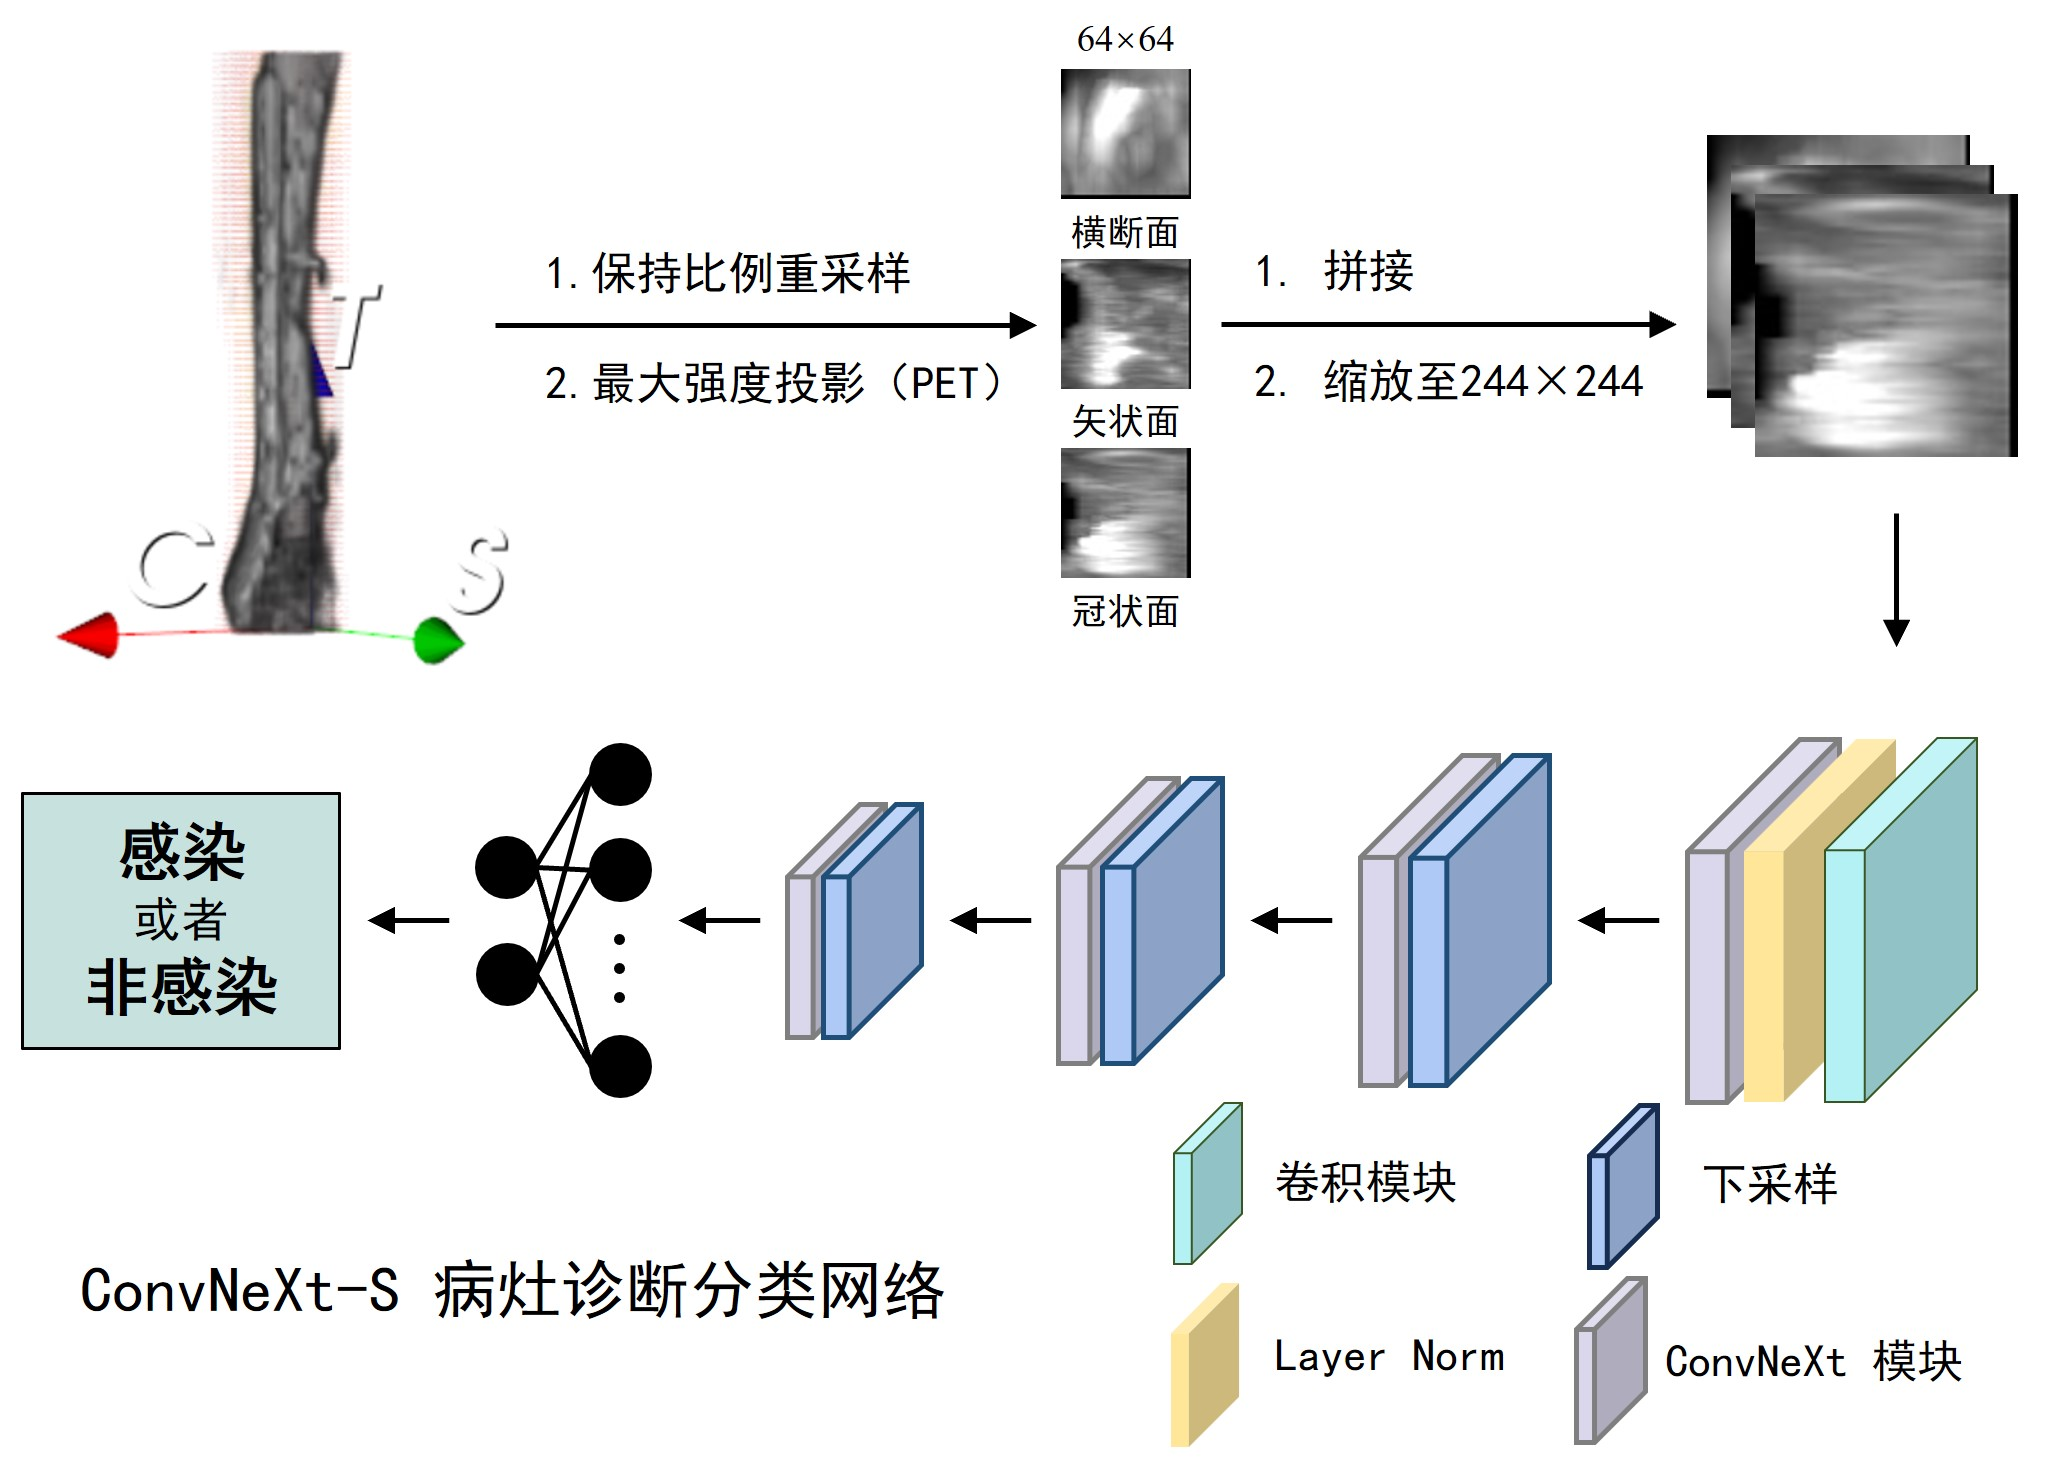
\includegraphics[width=0.6\textwidth]{figures/chap04_classifier.jpg}
    \caption{病灶诊断分类网络}
    \label{fig:chap04_classifier}
\end{figure}

首先,设置置信度阈值为0.1,最大输出的检测框数量为100,让目标检测网络322-YOLO输出所有符合条件的预测框。然后,设置交并比阈值为0.01,去除掉相同类别下重叠程度高于交并比阈值的预测框。最后,筛选得到类别为病灶的预测框。

根据得到的病灶预测框,在预处理后的PET影像上进行裁剪,得到病灶区域的PET影像。然后对病灶区域的PET影像进行等比例的缩放并在四周进行填充,使得最终获得的PET影像为\(64\times64\times64\)的大小,并将PET的SUV中小于0的设置为0。其中,PET中填充区域的值为0。在矢状轴、冠状轴和横断轴上进行最大强度投影得到的三张单通道图像拼接成一张三通道图像,并重采样至\(244 \times 244\)的大小后,输入到病灶诊断分类网络ConvNeXt-S之中,对病灶区域进行诊断分类,如图\ref{fig:chap04_classifier}所示。

将训练模型的图像输入到ConvNeXt-S诊断分类网络中,经过ConvNeXt-S的卷积层、Layer norm层、ConvNeXt模块、下采样层、平均池化层和全连接层得到最终的诊断分类结果。其中,在训练过程中,使用了镜像(水平或翻转)和Mixup来弥补数据集不足的问题,损失函数采用的是焦点损失函数(Focal Loss)。

\section{实验}

\subsection{实验环境}

本章所有实验均使用PAI上海大学机器学习平台上进行。学习平台配置:两个NVIDIA Tesla V100(32GB) GPU;Linux Ubuntu 20.04.2 操作系统;Pytorch 1.8.0 深度学习框架;Python 3.8.17 编程语言。具体详细的配置信息与上一章节一致。

\subsection{数据集}

\begin{table}[htbp]
    \centering
    \caption{下肢骨折相关感染的PET/CT影像数据集特征}
    \begin{tabular}{lc}
        \toprule
        特征         & 数量       \\
        \midrule
        骨折类别,数量(\%)      \\
        \quad 股骨   & 91 (30.5)  \\
        \quad 胫腓骨 & 169 (56.7) \\
        \quad 足     & 36 (12.1)  \\
        \quad 下肢   & 2 (0.7)    \\
        诊断结果,数量(\%)      \\
        \quad 感染   & 190 (63.8) \\
        \quad 非感染 & 108 (36.2) \\
        \bottomrule
    \end{tabular}
    \label{tab:chap04_dataset}
\end{table}

本章采用的下肢骨折相关感染的PET/CT影像数据集由本文作者与上海市第六人民医院核医学科合作构建。纳入数据集的标准:存在既往的下肢骨折手术治疗;存在术后症状,如疼痛、活动受限或红肿;进行过\(^{18}\)F-FDG PET/CT扫描;\(^{18}\)F-FDG PET/CT扫描时间与既往手术之间的时间间隔超过3个月;\(^{18}\)F-FDG PET/CT扫描时间与手术后的时间间隔少于1个月。排除标准:存在鼻窦道、脓等典型感染的临床表现;术后未行常规细菌培养以及病理分析;\(^{18}\)F-FDG PET/CT扫描前一周内使用抗生素;不完整的临床数据;现有资料不能确定最终诊断。在数据集方面,一共纳入了从2016年11月到2021年12月之间303名潜在合格的患者。在阅览所有患者的PET/CT影像后,22名患者因为影像缺失或不完整被排除掉。最终,具有298个病灶区域的281名患者被纳入本章的研究中,详细信息如表\ref{tab:chap04_dataset}所示。本章研究中所有患者骨折相关感染的最终诊断是基于手术中深部组织提取后的医学微生物培养或组织病理学分析以及至少6个月的临床随访。

\subsection{评价指标}

假体关节感染任务包含目标检测和分类问题。在目标检测任务中,本章选用了平均精度(Average Precision,AP)、精确率(Precision)、召回率(Recall)和F1值(F1 score),如式\ref{eq:chap04_metric}所示。
\begin{equation}
    \begin{aligned}
        Precision & = \frac{TP}{TP+FP}                                                   \\
        Recall    & = \frac{TP}{TP+FN}                                                   \\
        F1 socre  & = \frac{2 \times Precision \times Recall}{Precision + Recall}        \\
        AP        & = \sum_{r_i}(Recall_{r_i} - Recall_{r_{i-1}}) \times Precision_{r_i} \\
    \end{aligned}
    \label{eq:chap04_metric}
\end{equation}
其中,\(TP\)(True Positive)是被正确检测为正类别的样本数量,\(FP\)(False Positive)是被错误检测为正类别的样本数量,\(FN\)(False Negative)是被错误地标记为负类别的样本数量。\(Recall_{r_i}, Precision_{r_i}\)表示根据模型输出和真实标签,在置信度为\(r_i\)下的精确率和召回率。平均精度衡量了在不同置信度阈值下目标检测网络的精确率和召回率之间的平衡,是一个综合性指标;精确率表示预测为正类别的样本中实际为正类别的比例;召回率表示实际为正类别的样本中被正确预测为正类别的比例。分类任务采用的评估指标有Acc,Spec,Sen,PPV,NPV,F1,AUC与上一个章节一致。Acc评估下肢假体关节感染的诊断准确率;Spec评估实际不患骨折相关感染的患者诊断未未感染的概率;Sen评估实际患有骨折相关感染的患者诊断为感染的概率。PPV评估被诊断为骨折相关感染的患者实际患有的概率;NPV评估被诊断未患骨折相关感染的患者实际未感染的概率。F1是PPV和Sen的综合评价指标,AUC是敏感性和特异性在不同阈值设定下生成的ROC曲线下的面积。

\subsection{实验结果}

\begin{table}[htbp]
    \centering
    \caption{病灶检测网络与YOLO系列模型在病灶上的检测性能比较}
    \resizebox{\textwidth}{!}{
        \begin{tabular}{lccccccccccc}
            \toprule
            模型     & AP\(_{25:75}\)  & AP\(_{25}\)     & Precision\(_{25}\) & Recall\(_{25}\) & F1\(_{25}\)     & AP\(_{50}\)     & Precision\(_{50}\) & Recall\(_{50}\) & F1\(_{50}\)     & flops   & params  \\
            \midrule
            YOLOv3   & 0.1941          & 0.5656          & 0.6842             & 0.6290          & 0.6566          & 0.1152          & 0.1579             & 0.1452          & 0.1515          & 368.79G & 172.95M \\
            YOLOv4   & 0.2553          & 0.7377          & 0.8000             & 0.7742          & 0.7871          & 0.1405          & 0.2667             & 0.2581          & 0.2624          & 278.54G & 170.69M \\
            YOLOv5-S & 0.2019          & 0.6876          & 0.7377             & 0.7258          & 0.7318          & 0.0540          & 0.1803             & 0.1774          & 0.1789          & 35.65G  & 15.84M  \\
            YOLOv5-M & 0.2475          & 0.7265          & 0.7460             & 0.7581          & 0.7520          & 0.1644          & 0.3016             & 0.3065          & 0.3040          & 99.17G  & 50.12M  \\
            YOLOv5-L & 0.2113          & 0.7109          & 0.6957             & 0.7742          & 0.7349          & 0.0963          & 0.1884             & 0.2097          & 0.1990          & 216.93G & 114.87M \\
            YOLOX-S  & 0.3286          & 0.8085          & 0.8154             & 0.8548          & 0.8351          & 0.3032          & \textbf{0.4154}    & 0.4355          & \textbf{0.4254} & 59.15G  & 21.24M  \\
            YOLOX-M  & 0.3673          & 0.8049          & \textbf{0.8281}    & 0.8548          & 0.8415          & \textbf{0.3073} & 0.4063             & 0.4194          & 0.4128          & 152.03G & 62.29M  \\
            YOLOX-L  & 0.3069          & 0.7892          & 0.8000             & 0.8387          & 0.8194          & 0.1738          & 0.3077             & 0.3226          & 0.3151          & 310.91G & 136.53M \\
            322-YOLO & \textbf{0.3834} & \textbf{0.9234} & 0.8000             & \textbf{0.9677} & \textbf{0.8839} & 0.3041          & 0.3600             & \textbf{0.4355} & 0.3977          & 63.71G  & 26.04M  \\
            \bottomrule
            \multicolumn{12}{l}{\footnotesize *\(_{25:75}\)表示在IoU\(\in [0.25,0.75]\)以0.05为步长时*的平均值;*\(_{25}\)表示在IoU=0.25时*;*\(_{50}\)表示在IoU=0.50时*;}
        \end{tabular}
    }
    \label{tab:chao04_experiment_yolo}
\end{table}

本章提出的病灶检测网络322-YOLO跟其他YOLO系列模型的病灶检测性能进行了比较,如表\ref{tab:chao04_experiment_yolo}所示。其中,为了YOLO系列模型适用于三维的PET/CT影像数据,将YOLO系列模型的预处理、模型结构、后处理部分中都从相应的二维操作修改为了三维操作。在综合检测性能上,322-YOLO不仅拥有较小的计算量和参数量,还表现出了最佳的病灶定位检测性能。此外,322-YOLO的计算量和参数量还不到在AP\(_{25:75}\)上排名第二的YOLOX-M的一半。在其他关于病灶检测性能的细分评估指标AP\(_{25}\)、Recall\(_{25}\)、F1\(_{25}\)和Recall\(_{50}\)中,322-YOLO都是最佳的。这表明322-YOLO在病灶检测、计算量和参数量上的综合表现能力最佳。值得说明的是,322-YOLO在验证集中检测到了75个病灶区域,其中有63个与专业医生标记的病灶区域相匹配,有9个是未标记的骨折相干感染病灶区域,只有3个是完全误检。

\begin{table}[htbp]
    \centering
    \caption{病灶检测网络322-YOLO的消融实验}
    \resizebox{\textwidth}{!}{
        \begin{tabular}{lcccccccc}
            \toprule
                                & \multicolumn{3}{c}{病灶} & \multicolumn{3}{c}{膀胱} & \multirow{2}{*}{flops} & \multirow{2}{*}{params}                                                       \\
                                & AP\(_{25:75}\)           & AP\(_{25}\)              & AP\(_{50}\)            & AP\(_{25:75}\)          & AP\(_{25}\)     & AP\(_{50}\)     &        &        \\
            \hline\hline
            YOLOX-S             & 0.3286                   & 0.8085                   & 0.3032                 & 0.7676                  & 1.0000          & 0.8418          & 59.15G & 21.24M \\
            \midrule
            + SPP→SPPF*         & 0.3390                   & 0.7829                   & 0.2812                 & 0.7543                  & 1.0000          & 0.8870          & 59.15G & 21.24M \\
            + only use P4/P5    & 0.3248                   & 0.8506                   & 0.1650                 & 0.7714                  & 1.0000          & 0.8487          & 35.08G & 18.22M \\
            + SE block          & 0.3610                   & 0.8943                   & 0.1965                 & 0.7523                  & 1.0000          & 0.8355          & 35.09G & 18.24M \\
            + two path backbone & 0.3895                   & 0.9105                   & 0.2746                 & 0.7442                  & 0.9643          & 0.8857          & 63.71G & 26.04M \\
            + Mixup             & \textbf{0.4084}          & 0.9010                   & 0.2795                 & 0.7341                  & 1.0000          & 0.8615          & 63.71G & 26.04M \\
            + RICAP             & 0.3834                   & \textbf{0.9234}          & \textbf{0.3041}        & 0.7456                  & \textbf{1.0000} & \textbf{0.9279} & 63.71G & 26.04M \\
            \bottomrule
        \end{tabular}
    }
    \label{tab:chao04_experiment_ablation}
\end{table}

为了验证病灶检测网络中多个改进方法的有效性,如模型结构、数据增强,本章设计了消融实验。实验步骤如下:1.采用YOLOX-S作为基准模型对下肢骨折相关感染PET/CT影像数据集进行训练验证;2.在1的基础上,将主干网络中最后一个阶段的特征提取模块由SPP+CSP的组合修改为CSP+SPPF的组合,即+ SPP→SPPF*;3.在2的基础上,仅采用主干网络中提取的P4和P5特征图,颈部网络和头部网络结构也进行相应的修改,即+ only use P4/P5;4.在3的基础上,在主干网络部分添加通道注意力模型模块(Squeeze and Excitation Block),即+ SE block;5.在4的基础上,将主干网络从单分支修改为双分支的结构设计,即+ two path backbone;6.在5的基础上,训练过程中动态地随机使用适应性修改的Mixup数据增强方法,即+ Mixup;7.在6的基础上,训练过程中再动态地随机使用适应性修改的RICAP数据增强方法,即+ RICAP。在表\ref{tab:chao04_experiment_ablation}中可以看出,在综合检测性能指标AP\(_{25:75}\)中,除了+ only use P4/P5以外,所有在模型结构上的改进方法对病灶检测网络的病灶检测性能都有所提升。对于+ only use P4/P5而言,计算量和参数量的减少,使得病灶检测性能上的下降是可以接受的。数据增强方法Mixup在AP\(_{25:75}\)上进一步提升了模型检测病灶的能力,而RICAP在AP\(_{25}\)和AP\(_{50}\)上进一步达到了最优的结果。通过病灶检测网络的消融实验可以得出,病灶检测性能AP\(_{25:75}\)提升了16.7\%,AP\(_{25}\)达到了0.9234,AP\(_{50}\)达到了0.3041,这表明了本章研究中针对病灶检测任务提出的所有改进方法的有效性。

\begin{table}[htbp]
    \centering
    \caption{带额外分类器的病灶检测网络与单一病灶检测网络的性能比较}
    \begin{tabular}{ccccccc}
        \toprule
                              & \multicolumn{3}{c}{感染} & \multicolumn{3}{c}{非感染}                                                               \\
                              & AP\(_{25}\)              & AP\(_{50}\)                & AP\(_{25:75}\) & AP\(_{25}\) & AP\(_{50}\) & AP\(_{25:75}\) \\
        \midrule
        322-YOLO              & 0.6395                   & 0.3108                     & 0.3129         & 0.2193      & 0.0022      & 0.0433         \\
        322-YOLO + Classifier & 0.8016                   & 0.3346                     & 0.3790         & 0.6330      & 0.1253      & 0.1808         \\
        \bottomrule
    \end{tabular}
    \label{tab:chao04_experiment_1vs2}
\end{table}

为了验证单阶段算法与双阶段算法的效果差异,进行了对比实验,如表\ref{tab:chao04_experiment_1vs2}所示。如果仅使用322-YOLO自身的类别预测来进一步细分病灶类别,病灶的检测效果较差。而采用两阶段的病灶检测诊断分类网络框架3DFRINet(322-YOLO + Classifier),即通过添加二阶段的病灶诊断分类网络对已定位的病灶进行进一步地细分,可以大大的提高病灶检测性能。与单阶段的322-YOLO的病灶检测性能相比,3DFRINet在感染病灶中的AP\(_{25}\)、AP\(_{50}\)和AP\(_{25:75}\)分别提升了25.35\%、7.66\%和21.12\%,在非感染病灶中的AP\(_{25}\)、AP\(_{50}\)和AP\(_{25:75}\)分别提升了188.65\%、5595.45\%和317.55\%。这进一步证明了添加一个额外的仅关注于病灶区域的分类器效果更好。

\begin{table}[htbp]
    \centering
    \caption{两阶段检测诊断框架3DFRINet与6名核医学医生的比较}
    \resizebox{\textwidth}{!}{
        \begin{tabular}{ccccccccc}
            \toprule
                                      & Acc                & Spec               & Sen                & NPV                & PPV     & F1     & AUC    & \textit{p}      \\
            \hline\hline
            \multirow{2}{*}{3DFRINet} & 91.55\%            & 90.32\%            & 92.50\%            & 90.32\%            & 92.50\% & 0.9250 & 0.9331
                                      & \multirow{2}{*}{-}                                                                                                              \\
                                      & (83.10\%,97.18\%)  & (77.78\%,100.00\%) & (83.72\%,100.00\%) & (78.57\%,100.00\%) &
            (82.93\%,100.00\%)        & (0.8533,0.9756)    & (0.8547,0.9870)                                                                                            \\
            \midrule
            Junior 1                  & 74.65\%            & 93.55\%            & 60.00\%            & 64.44\%            & 92.31\% & 0.7273 & -      & \textbf{0.0018} \\
            Junior 2                  & 80.28\%            & 80.65\%            & 80.00\%            & 75.76\%            & 84.21\% & 0.8205 & -      & 0.0768          \\
            Junior 3                  & 74.65\%            & 77.42\%            & 72.50\%            & 68.57\%            & 80.56\% & 0.7632 & -      & \textbf{0.0075} \\
            Senior 1                  & 87.32\%            & 90.32\%            & 85.00\%            & 82.35\%            & 91.89\% & 0.8831 & -      & 0.4531          \\
            Senior 2                  & 85.92\%            & 90.32\%            & 82.50\%            & 80.00\%            & 91.67\% & 0.8684 & -      & 0.2188          \\
            Senior 3                  & 87.32\%            & 93.55\%            & 82.50\%            & 80.56\%            & 94.29\% & 0.8800 & -      & 0.3750          \\
            \bottomrule
        \end{tabular}
    }
    \label{tab:chao04_experiment_physician}
\end{table}

为了进行更加全面的对比评估实验,本章将提出的两阶段的病灶检测诊断分类网络框架3DFRINet与6名核医学影像科的临床医生进行比较。其中,有3名初级核医学医师和3名高级核医学医师。表\ref{tab:chao04_experiment_physician}展示了提出的3DFRINet的分类性能评估指标及其95\%的置信区间和6名核医学医师的诊断性能表现。从对比结果可以得出,3DFRINet拥有91.55\%的准确率、92.50\%的敏感率、90.32\%的阴性预测值和0.9250的F1上,均优于3名初级核医学医师和3名高级核医学医师。此外,其90.32\%特异率和92.50\%的阳性预测值都位列前三。这表明了3DFRINet相比较于3名初级核医学医师和3名高级核医学医师具有优秀的骨折相关感染诊断分类的性能表现。通过统计学分析,3DFRINet与两名初级核医学医生在准确率上的p值小于0.05,这说明3DFRINet与两名初级核医学医生在准确率上存在显著差异,而与1名初级核医学医师和3名高级核医学医师在准确率无显著差异。由此可知,3DFRINet具有与初级核医学医生更好或相同的诊断能力,与高级核医学医生相当的诊断性能。

\begin{figure}[htbp]
    \centering
    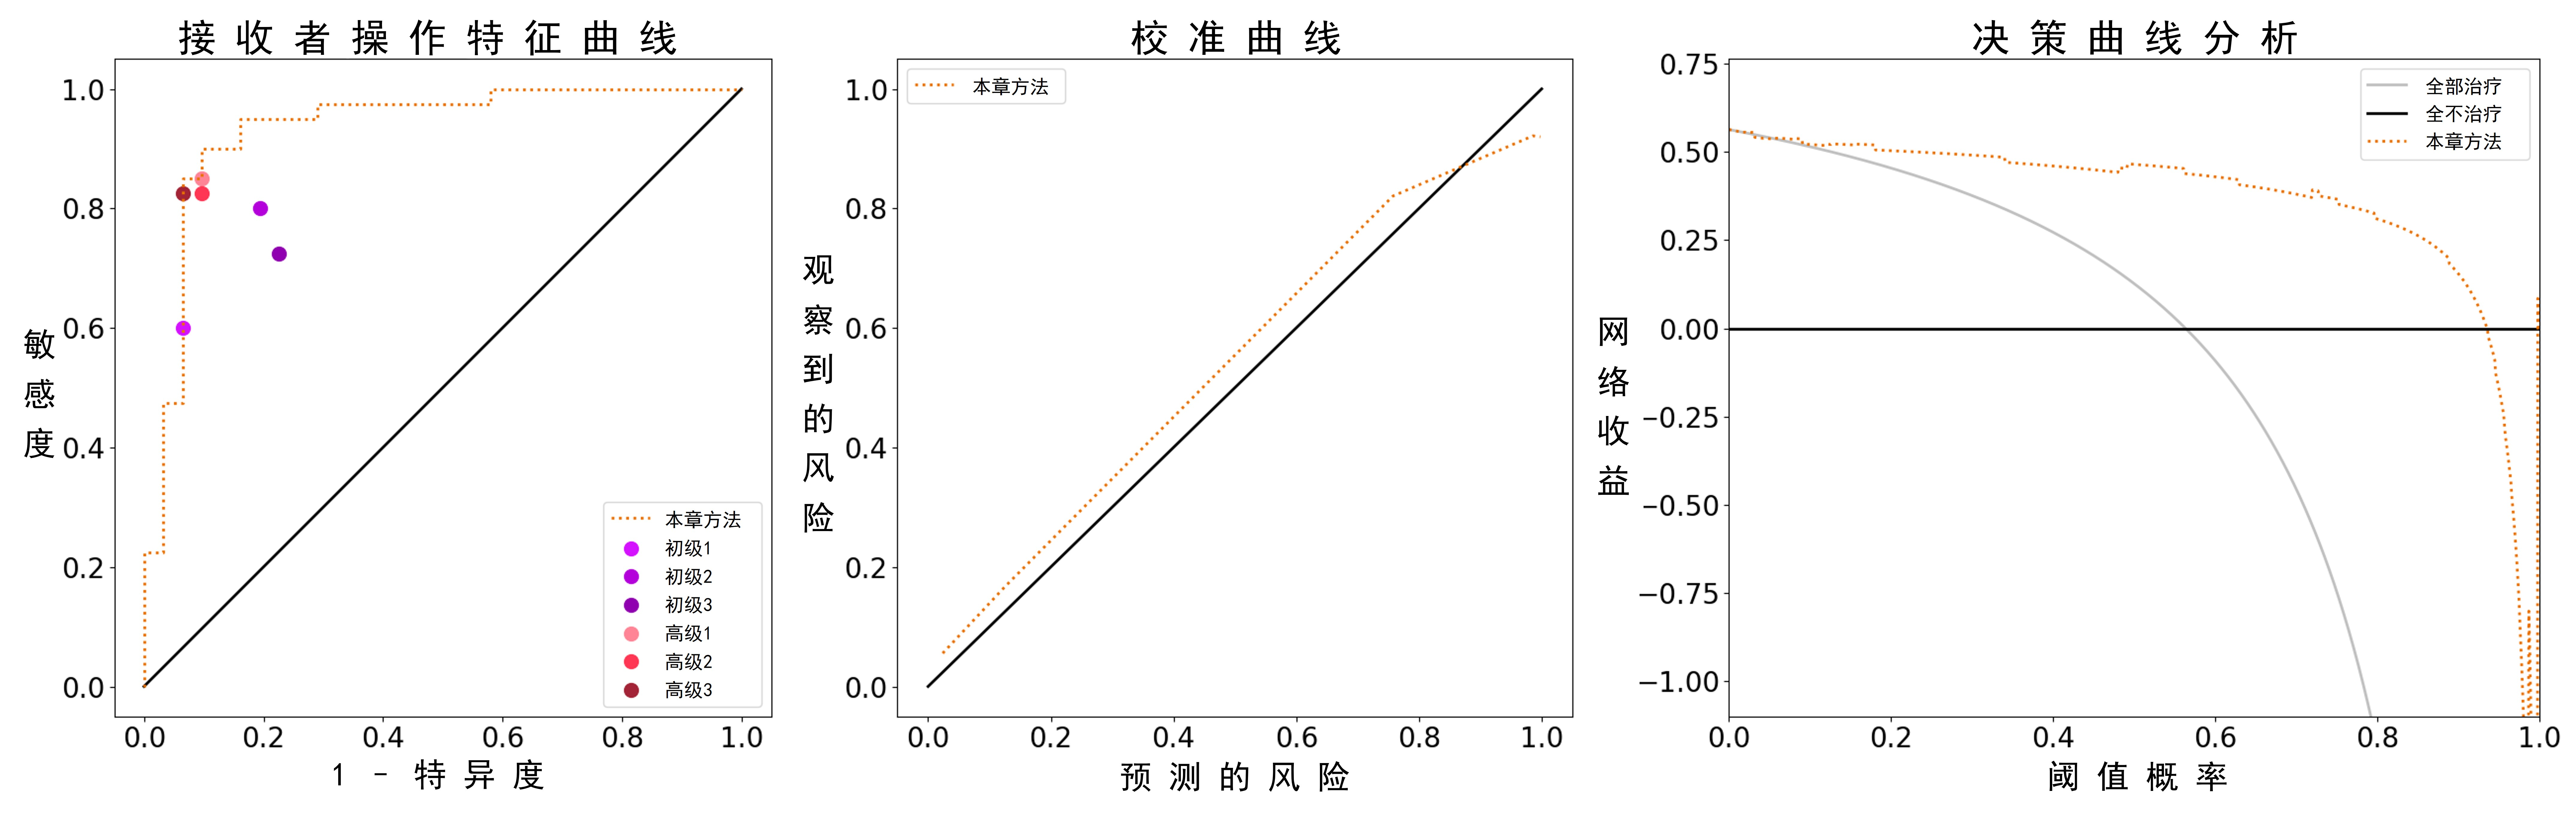
\includegraphics[width=\textwidth]{figures/chap04_eval.jpg}
    \caption{6名核医学医生与3DFRINet的ROC曲线;3DFRINet的标准曲线和决策曲线分析;}
    \label{fig:chap04_eval}
\end{figure}

如图\ref{fig:chap04_eval}所示,从ROC曲线上可以得出3DFRINet的诊断分类性能与三名高级核医学医师相当。3DFRINet的校准曲线较接近与45度对角线,这反映了在三维PET/CT影像上骨折相关感染的预测概率与骨折相关感染的真是改了具有良好的一致性。3DFRINet的决策曲线分析显示,网络在阈值概率较高的情况下存在负面收益,但大多数情况下是存在收益的且有价值的。

\subsection{可视化分析}
\begin{figure}
    \centering
    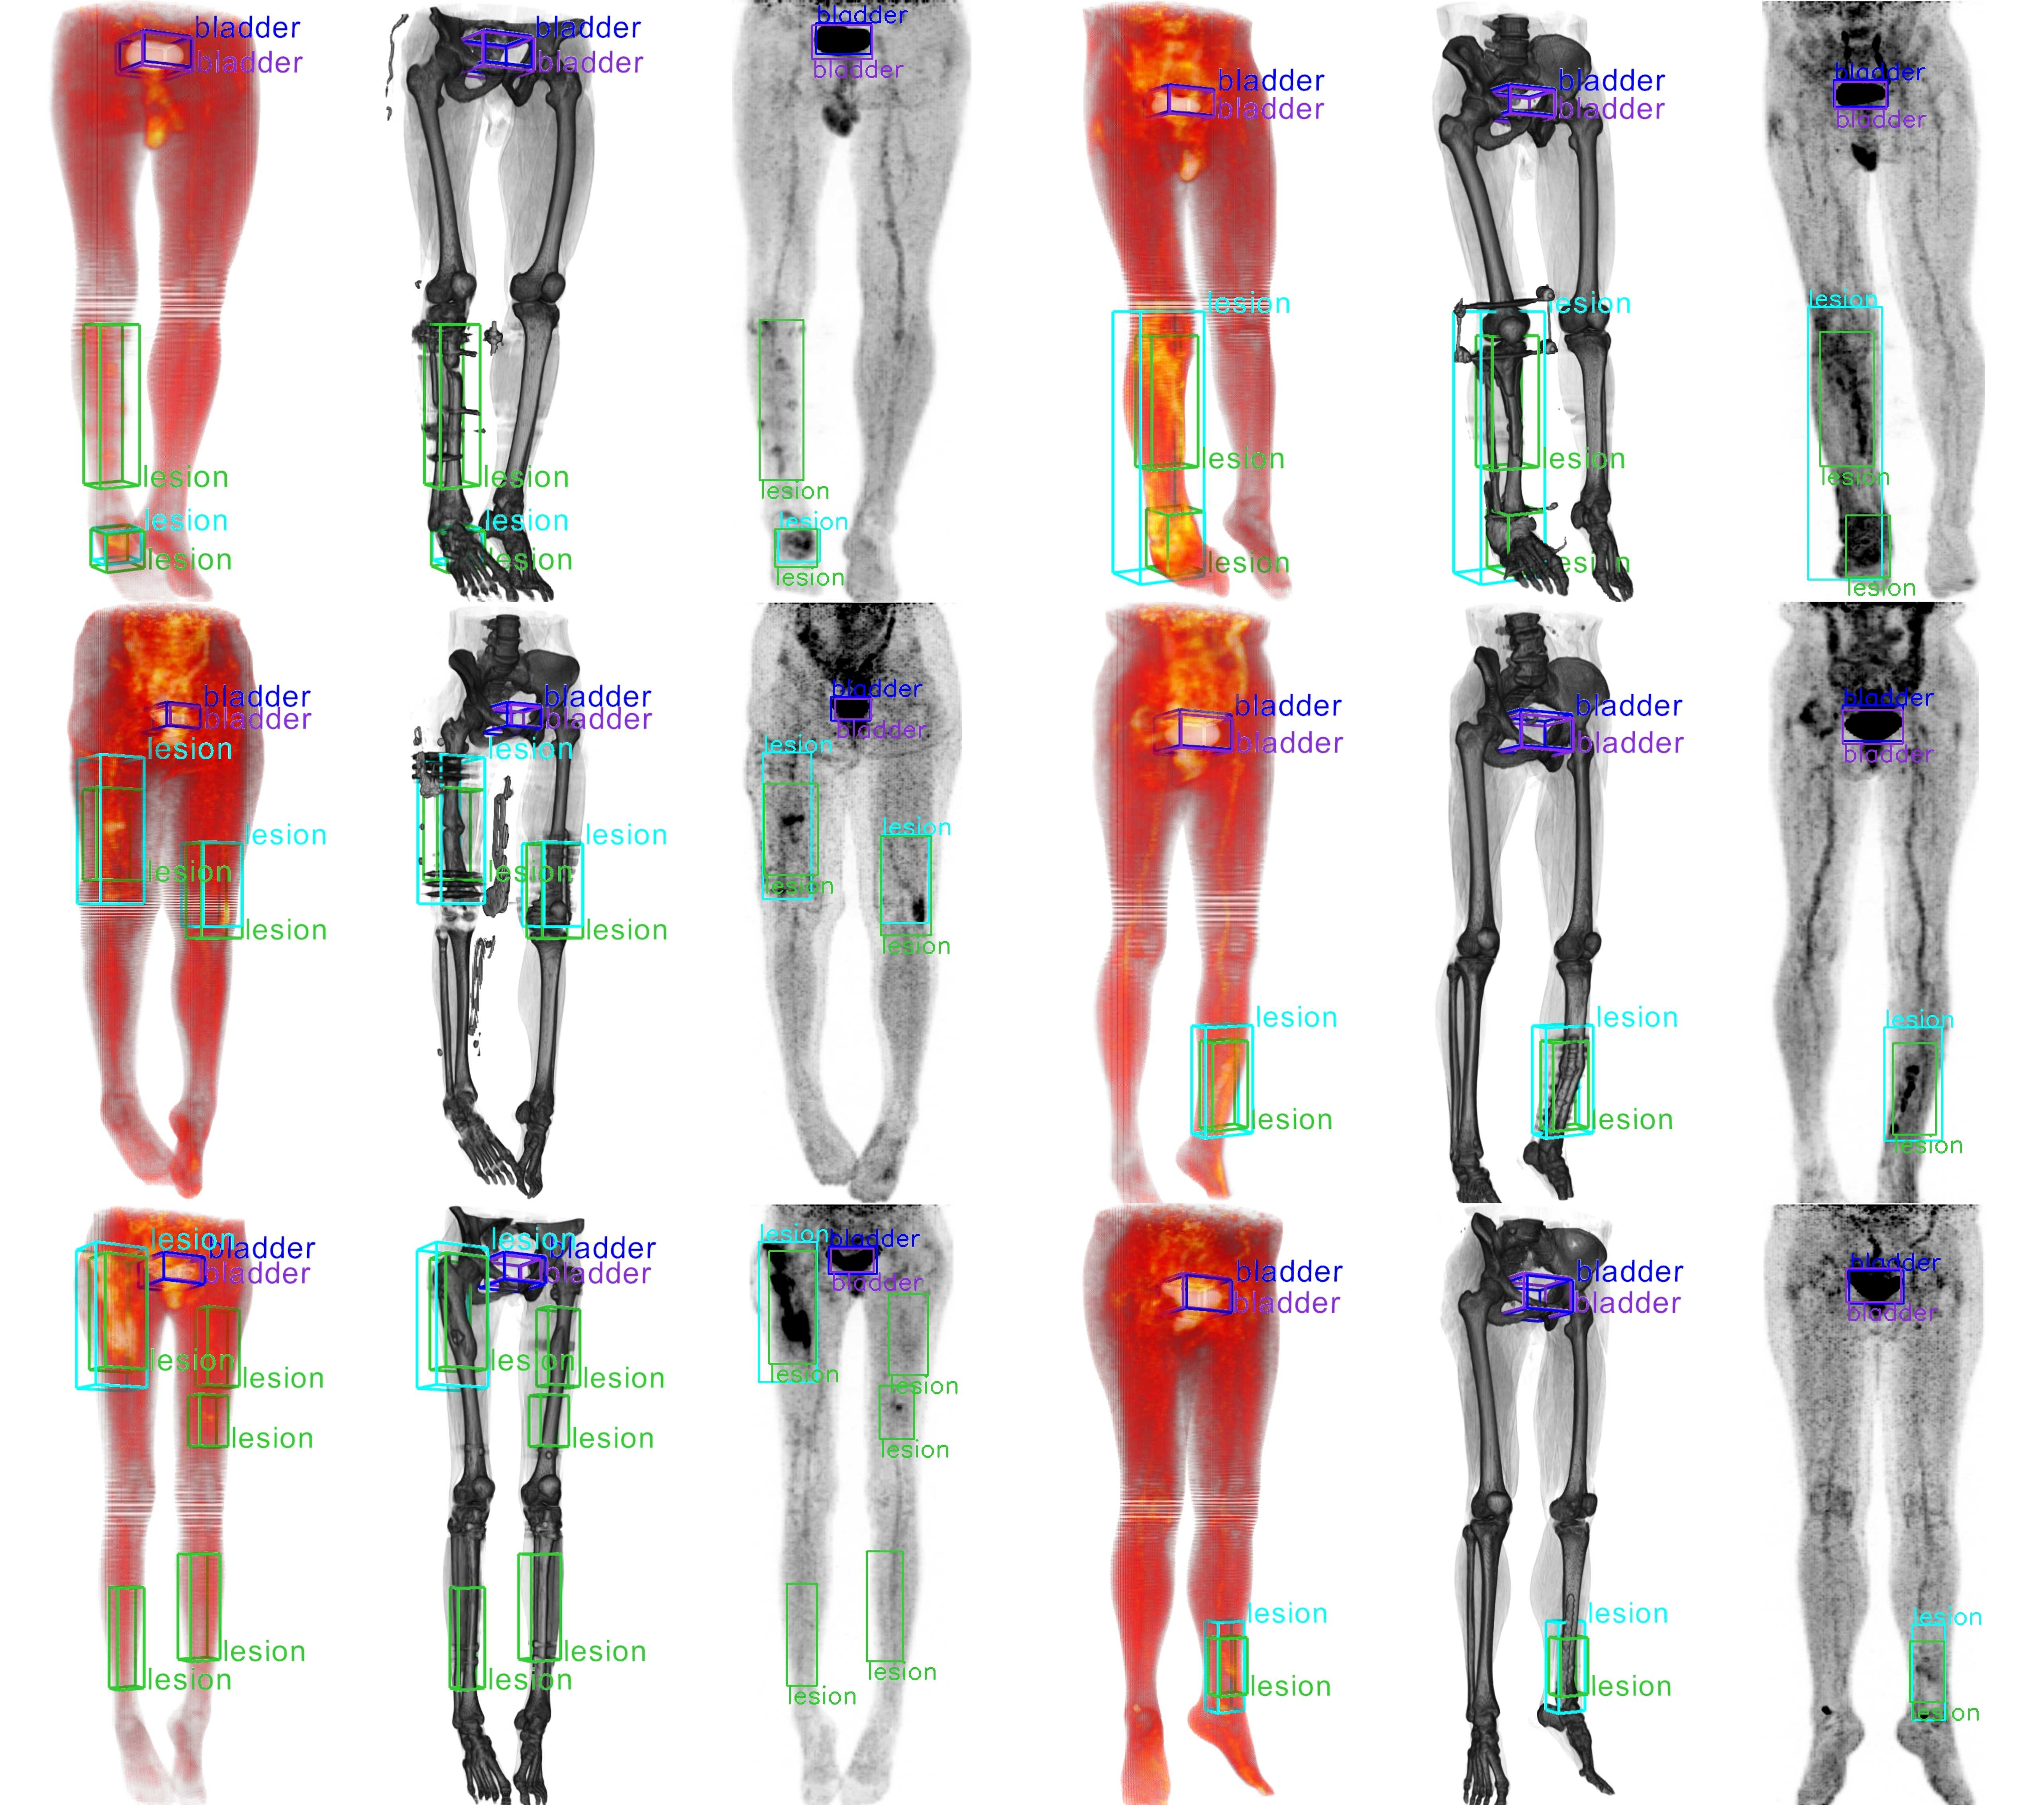
\includegraphics[width=\textwidth,height=\textheight,keepaspectratio]{figures/chap04_vis.jpg}
    \caption{322-YOLO检测结果的可视化图:每个患者有最大强度投影图像(PET),点云(3D PET)和三维重建的CT。青色和蓝色表示真实标签,紫色和绿色表示检测结果}
    \label{fig:chap04_vis}
\end{figure}

如图\ref{fig:chap04_vis}所示,322-YOLO展现了出色的性能,不仅能够准确定位已标注的病灶区域,而且能够有效检测出未标注的病灶区域(第1行第1列,第3行第1列)。特别值得注意的是,在病灶区域过大的情况下,322-YOLO还能通过使用两个边界框(第1行第2列)精准地定位病灶中更值得关注的子区域。此外,无论PET图像中是否存在高摄取区域,或者CT图像中是否存在骨侵蚀、骨折或内固定物等情况,322-YOLO模型都能够进行综合考虑并做出准确的检测与定位(第2行和第3行)。这表明了322-YOLO对于复杂场景和不同病变情况的强大适应性和鲁棒性。

\section{本章小结}

本章主要提出了一个基于\(^{18}\)F-FDG PET/CT影像的两阶段的下肢骨折相关感染病灶检测诊断分类网络框架3DFRINet,由预处理、322-YOLO病灶检测网络和ConvNeXt-S病灶诊断分类网络组成。预处理通过去除掉无关区域保留人体区域的PET SUV和CT HU输入到3DFRINet中。在322-YOLO病灶检测网络中,通过双分支主干网络结构设计与通道注意力模块有效地提取并融合三维PET的生理代谢信息和CT的解剖结构信息,从而充分利用不同模态的特点准确地检测病灶。通过最大强度投影将检测到的病灶从三维转换为二维,在降低数据和模型规模的同时获取有效特征,ConvNeXt-S病灶诊断分类网络达到了优异的分类性能。在下肢骨折相关感染的诊断任务中,该框架在检测方面达到了0.9234的AP\(_{25}\)和0.3041的AP\(_{50}\),在诊断分类方面达到了91.55\%(83.10\%,97.18\%)的准确率、0.9250(0.8533,0.9756)的F1和0.9331(0.8547,0.9870)的AUC,这表明该框架具有优越的病灶检测性能和良好的诊断分类性能。在与核医学医师的比较中,该框架相当或优于初级核医学医师,且与高级核医学医师相当。这进一步表现了深度学习方法在诊断假体关节感染的可行性与该病灶检测诊断分类网络框架的有效性。